\chapter{Evaluation}
\label{evaluation}
In diesem Kapitel wird nun genauer betrachtet, wie sich die Modelle unter Anwendung von Quantisierung und Pruning verhalten. Dazu werden als Erstes die Metriken besprochen, welche in dieser Arbeit als Grundlage für die Auswertung verwendet werden. Als Nächstes wird der Raspberry Pi 4 als Plattform für die Evaluation vorgestellt und besprochen, wie diese Plattform bei der Evaluation verwendet wird. Darauf folgt in einem weiteren Abschnitt die eigentliche Evaluation, bei der die Architekturen und Optimierungstechniken anhand der besprochenen Metriken ausgewertet und verglichen werden. Dabei wird zuerst auf das Training der Architekturen eingegangen. Anschließend werden nacheinander die Auswirkungen der Techniken Quantisierung und Pruning vorgestellt. Nach diesem Abschnitt folgt noch ein Abschnitt, der darauf eingeht, wie sich die Optimierungstechniken auf die einzelnen Klassen des CIFAR-10 Datensatzes auswirken. Als Letztes wird noch untersucht, inwieweit sich die Anwendung der besprochenen Optimierungstechniken auf die Architekturen optimieren lässt und welche Architekturen sich am besten für die Aufgabe der Bildklassifikation auf dem CIFAR-10 Datensatz eignen. 



\section{Metriken}
\label{metriken}
In diesem Abschnitt werden die Metriken beschrieben, die für jede der beschriebenen Architekturen erhoben wurden. Bei der Auswahl dieser Metriken ist es besonders wichtig darauf zu achten, dass die gewählten Metriken einen guten Einblick darin geben, wie sich die Architekturen verhalten, wenn die beschriebenen Optimierungstechniken angewendet werden. In dieser Arbeit wurden dafür insgesamt 5 Metriken ausgewählt, die im Folgenden genauer erläutert werden.


\subsection{Genauigkeit}
Als erste Metrik wird in dieser Arbeit die Genauigkeit der jeweiligen Modelle auf dem CIFAR-10 Datensatz (siehe Abschnitt \ref{datensatz}) betrachtet. Die Genauigkeit (Accuracy) beschreibt, gegeben einer Menge von $N_{all}$ Beispielen, wenn $N_{correct}$ Beispiele korrekt klassifiziert wurden, wie groß der Anteil der korrekt klassifizierten Beispiele ist. Somit ist diese Metrik bei einem Klassifizierungsproblem ein mögliches Maß dafür, wie gut ein trainiertes Modell die Klassifizierungsaufgabe bewältigt. Die Genauigkeit ist wie in Formel \ref{eq4.1} definiert:
\begin{eqnarray}
\textit{Accuracy} = \frac{N_{correct}}{N_{all}}
\label{eq4.1}
\end{eqnarray}

In dieser Arbeit wird für jede der Architekturen die sogenannte Top-1 und Top-3 Accuracy bestimmt. Jede der besprochenen Architekturen, die auf dem CIFAR-10 Datensatz trainiert wurden, liefern bei einer Inferenz einen Vektor mit jeweils einer Wahrscheinlichkeit pro Klasse. Damit wird modelliert, mit welcher Wahrscheinlichkeit, welche Klasse auf das zugrunde liegende Bild zutrifft. Betrachtet man bei der Inferenz nur die Klasse mit der höchsten Wahrscheinlichkeit und berechnet die Accuracy dafür, entspricht das der Top-1 Accuracy. Dies ist äquivalent mit der anfangs beschriebenen Definition. Bei der Berechnung der Top-3 Accuracy werden die Klassen mit den höchsten 3 Wahrscheinlichkeiten betrachtet und ein Bild gilt als korrekt klassifiziert, wenn sich die tatsächliche Klasse des Bildes unter den Klassen mit den höchsten 3 Wahrscheinlichkeiten befindet.

Bei der bisherigen Definition wurde die Genauigkeit immer klassenübergreifend betrachtet. Jedoch kann die Genauigkeit auch für jede Klasse separat berechnet werden, indem $N_{all}$ allen Beispielen einer Klasse entspricht und $N_{correct}$ allen richtig der Klasse zugeordneten Vorhersagen entspricht. Anschließend kann man mit der Formel \ref{eq4.1} die Accuracy berechnen.


\subsection{Parameteranzahl}
Eine weitere Metrik, welche in dieser Arbeit betrachtet wird, ist die Parameterzahl der einzelnen Modelle. Die Parameterzahl gibt Aufschluss über die Größe und Komplexität eines Modells und stellt ein gutes Maß dar, um Architekturen bzw. Modelle bezüglich der Größe untereinander zu vergleichen. Generell ist die Parameterzahl für eine bestimmte Architektur eine feste Kenngröße, die sich auch nicht durch ein Training verändert. Zusätzlich zu der einfachen Parameterzahl wird in dieser Arbeit aber auch die Sparsity der einzelnen Modelle betrachtet. Die Sparsity ist das Verhältnis zwischen der Anzahl der Parameter mit dem Wert 0 und der Gesamtanzahl aller Parameter. Diese Metrik beschreibt das Ausmaß eines Pruningvorgangs (siehe Abschnitt \ref{pruning}) und somit den Anteil an Parameter, welche keinen Einfluss mehr auf die Ausgabe des Netzes haben.


\subsection{Inferenzzeit}
Neben der Parameterzahl und der Genauigkeit ist die Inferenzzeit ebenfalls eine Metrik, welche im Kontext von mobilen/eingebetteten Systemen betrachtet werden sollte. Die Inferenzzeit beschreibt, wie viel Zeit ein Modell bei einer einzelnen gegebenen Eingabe für die Vorhersage benötigt. Durch die Anwendung von Optimierungstechniken, wie Quantisierung und Pruning, kann diese Inferenzzeit variieren und ist damit ebenfalls eine mögliche Metrik, um zu beschreiben, wie sich die Optimierungstechniken auf die gegebenen Architekturen auswirken. Wichtig ist bei der Erfassung der Inferenzzeit, dass eine einheitliche Plattform verwendet wird, da die Inferenzzeit eines Modells stark von den zur Verfügung stehenden Ressourcen der Plattform abhängt. In dieser Arbeit wird zum Erfassen der Inferenzzeit für jedes Modell ein Raspberry Pi 4 verwendet (siehe Abschnitt \ref{raspberry_pi_4}) und die Inferenzzeit wird mittels des TensorFlow Benchmark Tool bestimmt (siehe Abschnitt \ref{tensorflow_benchmark_tool}).


\subsection{Bedarf an Hintergrundspeicher}
Besonders im Bereich von mobilen und eingebetteten Systemen ist eine wichtige Metrik der Bedarf an Hintergrundspeicher eines Modells, da dieser in diesem Anwendungskontext häufig limitiert ist. Der Bedarf an Hintergrundspeicher kann durch Optimierungen, wie Quantisierung, deutlich reduziert werden, womit der Bedarf an Hintergrundspeicher ebenfalls bei der Beurteilung der Optimierungstechniken berücksichtigt werden sollte. Um diese Metrik zu erheben, wird die Dateigröße der Modelle im TFLite FlatBuffer Format gemessen.


\subsection{Bedarf an Hauptspeicher}
Als letzte Metrik wird neben dem Bedarf an Hintergrundspeicher auch der Bedarf an Hauptspeicher gemessen. Dieser ist ebenfalls besonders im eingebetteten und mobilen Anwendungsszenario von Interesse, da ebenfalls wie der Hintergrundspeicher der Hauptspeicher oft stark limitiert ist. Zusätzlich ist es beispielsweise beim Hauptspeicher eines Smartphones nicht wünschenswert, wenn ein Modell den Großteil des Hauptspeichers ausnutzt und somit andere Prozesse nicht arbeiten können, bis das Modell wieder ausgelagert wird. Aus diesem Grund wird in dieser Arbeit ebenfalls untersucht, inwieweit sich der Hauptspeicherbedarf der Modelle unter Anwendung von Quantisierung und Pruning verändert. Gemessen wird der Hauptspeicherbedarf, genau wie die Inferenzzeit, auf dem Raspberry Pi 4 mittels des TensorFlow Benchmark Tools (siehe Abschnitt \ref{raspberry_pi_4} und \ref{tensorflow_benchmark_tool}).


\section{Raspberry Pi 4}
\label{raspberry_pi_4}
Insbesondere um die Inferenzzeit der einzelnen Modelle zu erfassen, wird eine einheitliche Plattform benötigt, um die Vergleichbarkeit der Ergebnisse sicherzustellen. In dieser Arbeit wird als Plattform ein Raspberry Pi 4 B \footnote{\url{https://www.raspberrypi.org/products/raspberry-pi-4-model-b/}} verwendet.

Bei dem Raspberry Pi 4 B handelt es sich um einen Single-Board Computer, welcher als Prozessor einen 64 Bit Quad-Core Cortex-A72 der ARMv8 Architektur mit 1.5GHz Taktfrequenz verwendet. Erhältlich ist der Raspberry Pi 4 in drei Varianten mit jeweils 2GB, 4GB oder 8GB Hauptspeicher. In dieser Arbeit wird der Raspberry Pi 4 mit 8 GB Hauptspeicher verwendet. Jedoch besitzt jede dieser Varianten genug Hauptspeicher für die betrachteten Architekturen (siehe Abschnitt \ref{ergebnisse}). Durch die geringe Größe von $88mm \times 58mm \times 19.5mm$ und der verhältnismäßig geringen Stromaufnahme im Ruhezustand von $600mA$ bei 5V Betriebsspannung lässt sich der Raspberry Pi vielseitig einsetzen und kann für einige eingebettete Anwendungen eine Option darstellen.

Als Betriebssystem für den Raspberry Pi 4 wird in dieser Arbeit Ubuntu Server 20.04 \footnote{\url{https://ubuntu.com/download/raspberry-pi}} verwendet.


\subsection{TensorFlow Benchmark Tool}
\label{tensorflow_benchmark_tool}
Um nun mittels des Raspberry Pi 4 sowohl die Inferenzzeit als auch den Bedarf an Hauptspeicher zu erfassen, wird in dieser Arbeit das von TensorFlow bereitgestellt Model Benchmark Tool \footnote{\url{https://github.com/tensorflow/tensorflow/tree/master/tensorflow/lite/tools/benchmark}} verwendet. Damit das Tool verwendet werden kann, muss es auf der Zielplattform (in diesem Fall der Raspberry Pi 4) kompiliert werden.

Bei diesem Tool handelt es sich um eine einfache C++ Binärdatei, welche als notwendiges Kommandozeilenargument den Pfad zu einem Modell im TFLite FlatBuffer Format erhält (\lstinline{--graph="Pfad/zum/tflite_model"}). Anschließend generiert das Modell zufällige Eingabedaten und lässt das Modell für jede generierte Eingabe eine Inferenz durchführen. Das Benchmark Tool misst dann für jede Inferenz die benötigte Zeit und bildet ein arithmetisches Mittel darüber. Für diese Messung wird zuerst eine festgelegte Anzahl an Warmup Runs durchgeführt. Diese Warmup Runs sind Inferenzen, bei denen noch nicht die Inferenzzeiten gemessen werden. Die Anzahl dieser Warmup Runs kann über das Kommandozeilenargument \lstinline{--warmup_runs} gesteuert werden. Standardmäßig wird ein einzelner Warmup Run durchgeführt. Auf diese Warmup Runs folgen die eigentlichen Durchläufe, deren Anzahl über das Argument \lstinline{--num_runs} gesteuert werden kann. Als Standardwert sind hier 50 Durchläufe festgelegt. Für die Anzahl an Warmup Runs und die Anzahl an Messdurchläufen werden in dieser Arbeit die Standardwerte verwendet.

Neben der Inferenzzeit erfasst das Benchmark Tool aber auch den Spitzenbedarf an Hauptspeicher des Modells. Dabei ist aber zu beachten, dass der Bedarf an Hauptspeicher, den das Tool ausgibt, lediglich eine Näherung ist, da das Tool selbst noch Hauptspeicher benötigt, welcher mit in den Wert einfließt.



\section{Ergebnisse}
\label{ergebnisse}
In diesem Abschnitt wird darauf eingegangen, wie sich die einzelnen Architekturen in den zuvor beschriebenen Implementierungsphasen Training, Quantisierung und Pruning verhalten. Dazu werden die zuvor beschriebenen Metriken ausgewertet und die resultierenden Ergebnisse diskutiert.

\subsection{Training}
\label{eval_training}
Nachdem die vorgestellten Netzwerkarchitekturen, wie in Abschnitt \ref{training} beschrieben, trainiert wurden, ergeben sich die in Tabelle \ref{t4.1} charakterisierten Modelle. Die Tabelle stellt die Parameterzahlen und Genauigkeiten auf den Trainings- und Testdaten der trainierten Modelle dar.

\begin{table}[ht]
\centering
\begin{tabular}{llllll}
\toprule
    Architekturen & Parameter &  Top-1 &  Top-3 &  Top-1 (Test) &  Top-3 (Test) \\
\midrule
        MobileNet &  3.2 Mio. & 0.8140 & 0.9650 &        0.7277 &        0.9226 \\
      MobileNetV2 &  2.3 Mio. & 0.8460 & 0.9715 &        0.7325 &        0.9263 \\
MobileNetV3 Large &  4.2 Mio. & 0.7749 & 0.9485 &        0.6934 &        0.9064 \\
MobileNetV3 Small &  1.5 Mio. & 0.7530 & 0.9451 &        0.6687 &        0.9033 \\
  EfficientNet-B0 &  4.1 Mio. & 0.8400 & 0.9694 &        0.7514 &        0.9296 \\
\bottomrule
\end{tabular}
\caption{Zusammenfassung der Genauigkeiten (Top-1 \& Top-3) auf den Trainings- und Testdaten nach dem Training und Parameterzahlen für jede Architektur.}
\label{t4.1}
\end{table}

Wie gut zu erkennen ist, tritt bei allen Modellen ein deutlich ausgeprägtes Overfitting auf, was sich daran erkennen lässt, dass die Genauigkeit der Modelle auf den Trainingsdaten um einiges höher ist als die Genauigkeit auf den Testdaten. Ein möglicher Grund für das Overfitting dieser Modelle könnte sein, dass der CIFAR-10 Datensatz mit den 10 Klassen und insgesamt 600000 Bildern verhältnismäßig klein ist für diese Architekturen mit mehreren Millionen Parametern. In den Veröffentlichungen zu den jeweiligen Architekturen \cite{howard_mobilenets_2017, sandler_mobilenetv2_2019, howard_searching_2019, tan_efficientnet_2020} wird der ImageNet Datensatz \cite{russakovsky_imagenet_2015} verwendet, welcher mit insgesamt 1431167 Bildern und 1000 Klassen um ein vielfaches größer ist als der in dieser Arbeit verwendete CIFAR-10 Datensatz.

Zusätzlich kann man in der Tabelle erkennen, dass das MobileNetV3 Large von der Parameterzahl die Größte der vorgestellten Architekturen ist. Jedoch ist beispielsweise das MobileNetV2 fast um die Hälfte kleiner was die Parameterzahl angeht, aber trotzdem ist die Top-1 Accuracy des MobileNetV2 auf den Testdaten um $5.6\%$ besser als das MobileNetV3 Large. Mögliche Gründe dafür könnten sein, dass zum einen die Architektur schlecht trainiert ist, da beim Training möglicherweise, für diese Architektur, ungünstige Parameter gewählt wurden. Zum anderen wurde in Abschnitt \ref{mobilenetv3} erwähnt, dass die letzten Schichten, welche für die Klassifizierung zuständig sind, für eine verringerte Latenz überarbeitet wurden. Dies könnte möglicherweise auch zu dem Genauigkeitsverlust gegenüber des MobileNetV2 beitragen. Ein weiterer Grund könnten die Squeeze-And-Excitation Schichten sein, die mit der MobileNetV3 Architektur hinzugefügt wurden. Jedoch nutzt das EfficientNet-B0 ebenfalls Squeeze-And-Excitation Schichten und diese Architektur hat die beste Genauigkeit von allen fünf betrachteten Architekturen.

\begin{table}[ht]
\centering
\begin{tabular}{lllll}
\toprule
    Architekturen & Parameter &  Datei [MB] &  RAM [MB] &  Inferenz [µs] \\
\midrule
        MobileNet &  3.2 Mio. &     12.8453 &   16.1016 &          11803 \\
      MobileNetV2 &  2.3 Mio. &      8.9153 &   11.2148 &           4961 \\
MobileNetV3 Large &  4.2 Mio. &     16.8829 &   20.4141 &           8051 \\
MobileNetV3 Small &  1.5 Mio. &      6.1536 &    8.5859 &           2954 \\
  EfficientNet-B0 &  4.1 Mio. &     16.0860 &   16.6719 &          12453 \\
\bottomrule
\end{tabular}
\caption{Auswertung der Metriken Dateigröße (Datei), Spitzen-Hauptspeicherbedarf (RAM) und Inferenzzeit (Inferenz) der trainierten Modelle auf dem Raspberry Pi 4.}
\label{t4.2}
\end{table}

Nachdem nun die Genauigkeiten der Architekturen diskutiert wurden, zeigt Tabelle \ref{t4.2} für jede der vorgestellten Architekturen die Parameterzahl, Dateigröße, Spitzen-Hauptspeicherbedarf und die Inferenzzeit auf dem Raspberry Pi 4. Vergleicht man nun die einzelnen Werte für jede Architektur untereinander, fällt auf, dass das MobileNetV3 Large im Spitzenwert deutlich mehr Hauptspeicher benötigt als das von der Größe (Parameterzahl und Dateigröße) vergleichbare EfficientNet-B0. Jedoch ist auf dem Raspberry Pi 4 die Inferenzzeit des EfficientNet-B0 $54.7\%$ höher als beim MobileNetV3 Large. Der Grund dafür ist vermutlich, dass die EfficientNet Architekturen in jedem der 16 Building Blocks ein Squeeze-And-Excitation Modul verwenden \cite{tan_efficientnet_2020} und diese Module noch nicht so gut unterstützt werden \cite{liu_higher_2020}. Aus diesem Grund haben die EfficientNet-Lite Architekturen (siehe Abschnitt \ref{efficientnet}) diese Squeeze-And-Excitation Module entfernt \cite{liu_higher_2020}. In den MobileNetV3 Architekturen werden Squeeze-And-Excitation Module deutlich weniger eingesetzt. Die MobileNetV3 Large Architektur verwendet lediglich 8 Squeeze-And-Excitation Module, was genau $50\%$ weniger sind als beim EfficientNet-B0.

Generell hat die kürzeste Inferenzzeit das MobileNetV3 Small mit $2954 \mu s$ und die längste Inferenzzeit hat das EfficientNet-B0 mit $12453 \mu s$.

Im weiteren Verlauf der Arbeit ist mit Top-1 und Top-3 Accuracy, wenn nicht anders gekennzeichnet, die Genauigkeit auf den Testdaten gemeint.


\subsection{Quantisierung}
\label{eval_quantisierung}
Wird auf die trainierten Modelle eine Post-Training Quantisierung angewendet, wie in Abschnitt \ref{impl_quantisierung} beschrieben, dann wird erwartet, dass sich vor allem die Dateigröße und der Hauptspeicherbedarf der quantisierten Modelle deutlich reduziert, da eine Quantisierung aller Parameter von 32 Bit Fließkommazahlen auf 8 Bit Integer durchgeführt wird. Damit wird die Größe der Parameter um das 4-fache reduziert. Zusätzlich wird durch die Reduzierung der Parameter von 32 Bit Fließkommazahlen auf 8 Bit Integer erwartet, dass durch die geringere Präzision der einzelnen Parameter die Genauigkeit der Modelle sinkt. In Tabelle \ref{t4.1} sind die Metriken der einzelnen Modelle nach Anwendung der Post-Training Float Fallback Quantisierung aufgelistet. Mit Top-1 und Top-3 ist (wie bereits in Abschnitt \ref{eval_training} erwähnt) die Genauigkeit auf den Testdaten gemeint.

\begin{table}[ht]
\centering
\begin{tabular}{lrrrrr}
\toprule
    Architekturen &  Top-1 &  Top-3 &  Datei [MB] &  RAM [MB] &  Inferenz [µs] \\
\midrule
        MobileNet & 0.7401 & 0.9312 &      3.6149 &   6.01560 &           3750 \\
      MobileNetV2 & 0.7507 & 0.9411 &      2.8626 &   6.91410 &           2843 \\
MobileNetV3 Large & 0.3963 & 0.7743 &      4.9440 &   6.93359 &           5259 \\
MobileNetV3 Small & 0.6349 & 0.8926 &      1.9539 &   5.20310 &           2183 \\
  EfficientNet-B0 & 0.7464 & 0.9324 &      5.1753 &   9.63670 &           8629 \\
\bottomrule
\end{tabular}
\caption{Metriken nach Anwendung von Quantisierung.}
\label{t4.3}
\end{table}

Zusätzlich ist in Abbildung \ref{f4.1} die prozentuale Veränderung der quantisierten Modelle gegenüber den Ausgangsmodellen nach dem Training dargestellt.

\begin{figure}[htbp]
\centerline{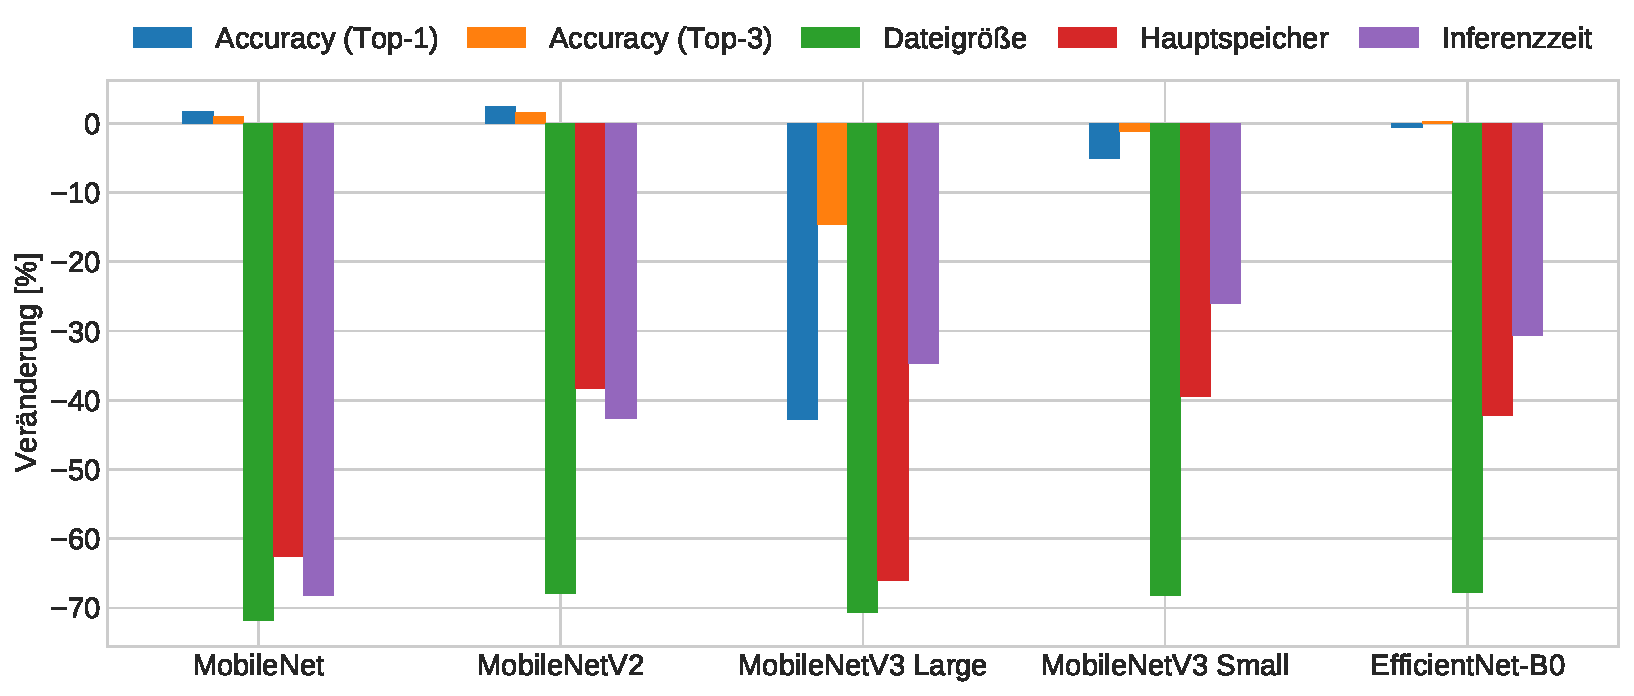
\includegraphics[width=\textwidth]{content/images/quantization_improvements.pdf}}
\caption{Prozentuale Veränderung der Metriken durch Anwendung von Quantisierung.}
\label{f4.1}
\end{figure}

Mit der Abbildung \ref{f4.1} wird sehr gut deutlich, wie sich die einzelnen Metriken bei der Anwendung von Quantisierung im Verhältnis zueinander verhalten und welche Kosten und welchen Nutzen eine Quantisierung dieser mobilen Architekturen beinhalten. Wie bereits am Anfang dieses Abschnittes diskutiert, lässt sich in Abbildung \ref{f4.1} erkennen, dass die Dateigröße der quantisierten Modelle gegenüber den nicht-quantisierten Modellen um ca. $70\%$ reduziert wird. Der Bedarf an Hauptspeicher und die Inferenzzeit werden je nach Architektur recht unterschiedlich beeinflusst. Es fällt jedoch auf, dass der Bedarf an Hauptspeicher bei der MobileNet und MobileNetV3 Large Architektur durch die Quantisierung um ungefähr $60\%$ reduziert werden kann. Die anderen Architekturen haben lediglich eine Reduktion von ungefähr $40\%$.

Bei der Diskussion der Auswirkung der Quantisierung auf die Genauigkeit am Anfang des Abschnittes wurde von einer Reduzierung der Genauigkeit ausgegangen. Jedoch zeigt Abbildung \ref{f4.1} und Tabelle \ref{t4.1}, dass die Genauigkeit nur sehr geringfügig beeinflusst wird. Tatsächlich verbessert sich sogar die Genauigkeit der MobileNet und MobileNetV2 Architektur um wenige Prozent. Die einzige Architektur, die bei der Quantisierung stark an Genauigkeit verloren hat, ist die MobileNetV3 Architektur. Die Top-1 Accuracy dieser Architektur ist durch die Quantisierung von $69.34\%$ auf $39.63\%$ abgefallen (siehe Tabelle \ref{t4.1}). Ein möglicher Grund für diesen Genauigkeitsverlust bei der Quantisierung der MobileNetV3 Large Architektur könnte sein, dass, wie im Abschnitt \ref{eval_training} bereits diskutiert, für das Training ungünstige Parameter gewählt wurden und somit diese Architektur schlecht trainiert ist. Durch dieses schlechte Training könnten möglicherweise einige Ausreißer in den Gewichten des Modells vorhanden sein, die für dieses schlechte Ergebnis bei der Quantisierung verantwortlich sind \cite{jacob_quantization_2017}. Damit eignet sich die MobileNetV3 Architektur bei dieser Trainingskonfiguration nicht für eine Post-Training Quantisierung.

Abgesehen von dem MobileNetV3 Large zeigen diese Ergebnisse, dass eine Post-Training Float Fallback Quantisierung der vorgestellten Architekturen mit wenig bis gar keinen Einbußen in der Genauigkeit durchgeführt werden kann. Jedoch sorgt diese Quantisierung für einen deutlich verringerten Bedarf an Hintergrundspeicher/Hauptspeicher und einer verringerten Inferenzzeit auf dem Raspberry Pi 4. Am meisten profitiert die MobileNet Architektur von der Quantisierung. Diese Architektur hat den Hintergrundspeicherbedarf, den Hauptspeicherbedarf und die Inferenzzeit um $62.6\%$ bis $71.9\%$ reduzieren können. Zusätzlich hat sich die Top-1 Accuracy um $1.7\%$ und die Top-3 Accuracy um $0.9\%$ gegenüber dem nicht quantisierten Modell verbessert.


\subsection{Pruning}
\label{eval_pruning}
Beim Pruning wird, wie bereits in Abschnitt \ref{impl_pruning} beschrieben, ein trainiertes Modell geladen und Schichten, die gepruned werden sollen, markiert. Anschließend werden, während eines erneuten Trainings auf dem bereits trainierten Modell, schrittweise Gewichte auf 0 gesetzt, die unter einen gewissen Schwellwert fallen. Nachdem dieses Vorgehen auf alle zu betrachteten Architekturen angewendet wurde, hat sich herausgestellt, dass der tatsächliche Anteil auf 0 gesetzter Gewichte (Sparsity) kleiner ist als der gewünschte Anteil. Der Grund dafür ist, dass TensorFlow beim Pruning den gewünschten Wert an Sparsity für jede markierte Schicht nur annähert. Zum anderen ist im Verlauf der Arbeit aufgefallen, dass in TensorFlow zum aktuellen Zeitpunkt zweidimensionale Depthwise Convolutions (\lstinline{tf.keras.layers.DepthwiseConv2D}) nicht gepruned werden. Das bedeutet, beim Markieren der \lstinline{DepthwiseConv2D} Schichten mittels der Funktion \lstinline{prune_layer}, wird die Schicht korrekt für das Pruning markiert. Jedoch werden im Verlauf des Pruningprozesses keine Gewichte dieser Schicht auf 0 gesetzt. Dieses Verhalten wurde zusätzlich in einem kleinen Minimalbeispiel verifiziert und Recherchen zu diesem Problem haben keine Lösung ergeben. Aus diesem Grund konnte das Problem in dieser Arbeit nicht behoben werden. Betrachtet man in Tabelle \ref{t4.4} die Anzahl an Parametern die durch die Depthwise Convolutions in die Architektur mit einfließen, kann man sehen, dass dies ein verhältnismäßig kleiner Anteil ist. Dieser kleine Anteil verringert aber trotzdem den Wert für die tatsächliche Sparsity.

\begin{table}[ht]
\centering
\begin{tabular}{llll}
\toprule
    Architekturen & Parameter & Parameter (Depthwise) & Anteil (Depthwise) \\
\midrule
        MobileNet &   3239114 &                 44640 &              1.38\% \\
      MobileNetV2 &   2270794 &                 64224 &              2.83\% \\
MobileNetV3 Large &   4239242 &                 91608 &              2.16\% \\
MobileNetV3 Small &   1540218 &                 58584 &              3.80\% \\
  EfficientNet-B0 &   4062381 &                182016 &              4.48\% \\
\bottomrule
\end{tabular}
\caption{Anteil an Parametern der Depthwise Convolutions zu der Gesamtparameterzahl der mobilen Architekturen.}
\label{t4.4}
\end{table}

Um sich der Frage nach den Auswirkungen von Pruning auf die mobilen Architekturen zu nähern, ist in Abbildung \ref{f4.2} die Top-1 Accuracy jeder Architektur für die verschiedenen exakten Sparsity-Werte nach dem Pruningvorgang dargestellt. Die $0\%$ Sparsity in der Abbildung \ref{f4.2} entsprechen den nicht geprunten Ausgangsmodellen nach dem erstmaligen Training. Wie in der Abbildung gut zu erkennen ist, verbessert sich bei allen Architekturen die Top-1 Accuracy, wenn die Architekturen auf $30\%$ Sparsity gepruned werden. Der Grund für die Verbesserung ist das erneute Training durch das Pruning und zusätzlich der geringe Anteil an Gewichten, die auf 0 gesetzt werden. Dadurch kann sich das Model leicht von den wenigen geprunten Gewichten erholen. Werden die Modelle auf $60\%$ gewünschte Sparsity gepruned, dann können das EfficientNet-B0 und das MobileNetV2 ihre ursprüngliche Genauigkeit ungefähr beibehalten. Das MobileNet und MobileNetV3 Large besitzen sogar bei $60\%$ Sparsity immer noch eine bessere Top-1 Accuracy als im nicht geprunten Zustand. Lediglich das MobileNetV3 Small hat sich leicht verschlechtert. Werden jedoch die Modelle auf $90\%$ gewünschte Sparsity gepruned, dann ergibt sich ein deutlich größerer Trade-Off. Alle Architekturen haben sich bei dieser Sparsity deutlich verschlechtert. Das MobileNetV3 Small verzeichnet nach diesem Pruningvorgang nur noch $46\%$ Top-1 Genauigkeit. Noch am besten hat dabei die MobileNet Architektur abgeschnitten, welche von einer Accuracy von $73\%$ auf eine Accuracy von $67\%$ abgefallen ist und damit bei einem Pruning mit $90\%$ gewünschter Sparsity von allen anderen betrachteten Architekturen die beste Genauigkeit aufweist.

\begin{figure}[htbp]
\centerline{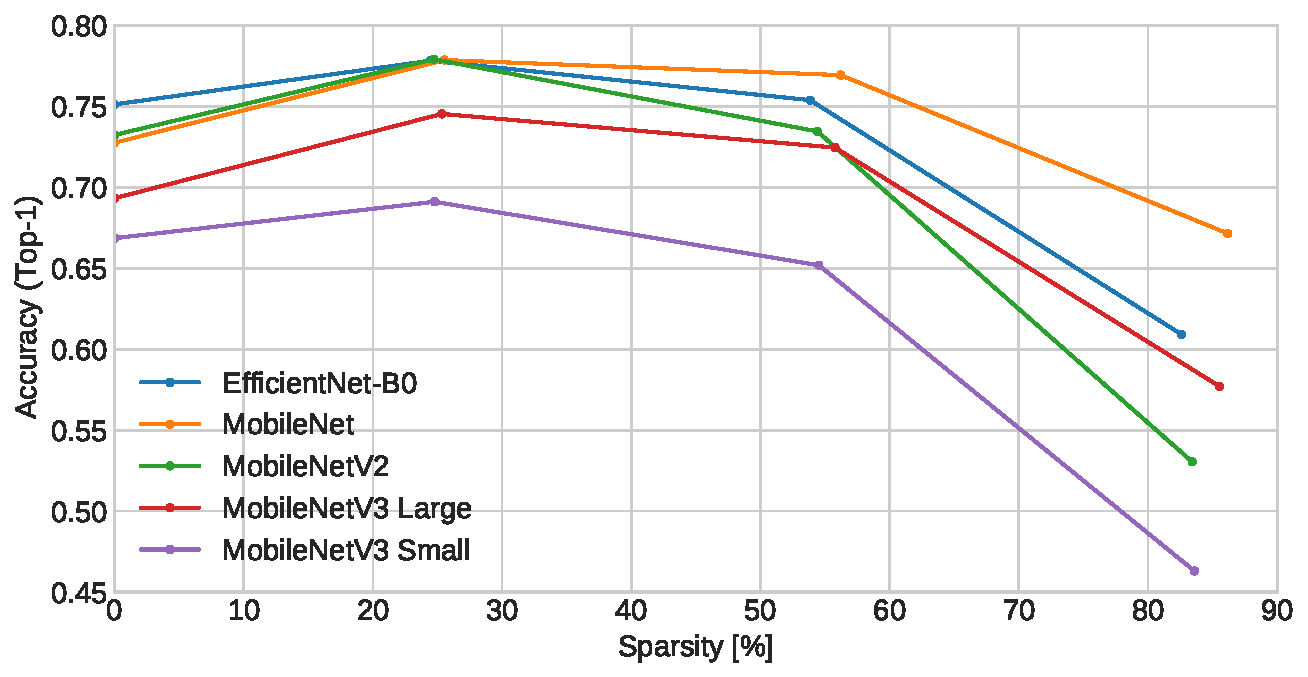
\includegraphics[width=0.8\textwidth]{content/images/sparsity_vs_accuracy.pdf}}
\caption{Genauigkeiten (Top-1) auf den Testdaten für die tatsächlichen Sparsity-Werte beim Pruning auf 0\% (ungepruned), 30\%, 60\% und 90\% Sparsity.}
\label{f4.2}
\end{figure}

Nach der Betrachtung der Genauigkeit stellt sich die Frage, welche Auswirkungen ein Pruning auf die restlichen betrachteten Metriken hat. Dazu ist in Tabelle \ref{t4.5} für jede Architektur und jede gewünschte Sparsity die tatsächliche Sparsity, der Hintergrundspeicherbedarf (Datei), der Bedarf an Hauptspeicher (RAM) und die Inferenzzeit aufgeführt. Was in dieser Tabelle sofort auffällt ist, dass die Metriken Hintergrundspeicherbedarf, Hauptspeicherbedarf und Inferenzzeit sich im Vergleich zu den nicht geprunten Ausgangsmodellen ($0\%$ Sparsity) in derselben Größenordnung befinden. Damit verbessert Pruning diese Metriken nicht.

Der Grund dafür, warum sich der Hauptspeicher- und Hintergrundspeicherbedarf nicht gegenüber den nicht-geprunten Modellen verändert, ist, dass beim Pruning die Gewichte nicht entfernt werden, sondern lediglich auf 0 gesetzt werden. Das bedeutet, bei einem 32 Bit Fließkomma-Modell (wie die trainierten Modelle in dieser Arbeit) werden beim Pruning die zu prunenden Gewichte auf die 32 Bit Fließkommazahl 0 gesetzt. Dadurch ergibt sich keine Speicherersparnis.

Zusätzlich wird in dieser Arbeit mit dem Magnitude Pruning ein unstrukturiertes Pruning betrieben, bei dem Gewichte an jeder beliebigen Stelle in dem Netzwerk gepruned werden können. Es wird beim unstrukturierten Pruning nicht darauf geachtet, die Gewichte in einer strukturierten Weise auf 0 zu setzen. Dies sorgt dafür, dass die aus dem unstrukturierten Pruning resultierenden Modelle nicht ohne weiteres bezüglich der Inferenzzeit optimiert werden können. Beim strukturierten Pruning hingegen werden ganze Neuronen, Filter oder Channel auf 0 gesetzt, was zu einer strukturierten Anordnung der geprunten Gewichten führt. Diese strukturiert geprunten Modelle können leichter durch Hardware und Software optimiert werden und können damit bessere Inferenzzeiten erreichen \cite{blalock_what_2020}.

\begin{table}[ht]
\centering
\begin{tabular}{llp{1.5cm}lll}
\toprule
Architekturen & Sparsity & Exakte Sparsity & Datei [MB] &  RAM [MB]  & Inferenz [µs]   \\
\midrule
MobileNet & 0\% &           0.00\% &     12.8453 &   16.1016 &          11803 \\
                & 30\% &          25.53\% &     12.8453 &   16.2148 &          11392 \\
                & 60\% &          56.21\% &     12.8453 &   16.1289 &          11594 \\
                & 90\% &          86.18\% &     12.8451 &   16.0625 &          11303 \\
\midrule
MobileNetV2 & 0\% &           0.00\% &      8.9153 &   11.2148 &           4961 \\
                & 30\% &          24.72\% &      8.9153 &   11.2656 &           4972 \\
                & 60\% &          54.41\% &      8.9153 &   11.2891 &           4933 \\
                & 90\% &          83.43\% &      8.9153 &   11.2617 &           4948 \\
\midrule
MobileNetV3 Large & 0\% &           0.00\% &     16.8829 &   20.4141 &           8051 \\
                & 30\% &          25.34\% &     16.8829 &   20.4180 &           7992 \\
                & 60\% &          55.78\% &     16.8829 &   20.3750 &           8098 \\
                & 90\% &          85.53\% &     16.8829 &   20.4727 &           8048 \\
\midrule
MobileNetV3 Small & 0\% &           0.00\% &      6.1536 &    8.5859 &           2954 \\
                & 30\% &          24.77\% &      6.1536 &    8.6211 &           2914 \\
                & 60\% &          54.52\% &      6.1536 &    8.6016 &           2959 \\
                & 90\% &          83.60\% &      6.1536 &    8.5898 &           2913 \\
\midrule
EfficientNet-B0 & 0\% &           0.00\% &     16.0860 &   16.6719 &          12453 \\
                & 30\% &          24.47\% &     16.0860 &   16.6484 &          12225 \\
                & 60\% &          53.86\% &     16.0860 &   16.5273 &          12376 \\
                & 90\% &          82.59\% &     16.0860 &   16.4492 &          12237 \\
\bottomrule
\end{tabular}
\caption{Zusammenfassung der exakten Sparsity, Dateigröße, Hauptspeicherbedarf und Inferenzzeit für die geprunten und unquantisierten Modelle.}
\label{t4.5}
\end{table}

Um aber trotzdem von den unstrukturiert geprunten Modellen zu profitieren, können die im \lstinline{.tflite}-Format gespeicherten Modelle mittels eines Kompressionsalgorithmus, wie gzip oder ZIP, komprimiert werden. Durch die hohe Anzahl an Gewichten mit dem Wert 0 sind diese Kompressionsalgorithmen in der Lage diese im TensorFlow Lite FlatBuffer gespeicherten Modelle stark zu komprimieren. Dieses Vorgehen wird so auch von dem Pruning-Guide \footnote{\url{https://www.tensorflow.org/model_optimization/guide/pruning/comprehensive_guide}} der TensorFlow Bibliothek vorgeschlagen. Abbildung \ref{f4.3} zeigt die Dateigröße der geprunten Modelle für jeden gewünschten Anteil an Sparsity nach Anwendung des gzip \footnote{\url{https://gzip.org/}} Kompressionsalgorithmus mit einem Kompressionslevel von 9. Der gzip Kompressionsalgorithmus wurde gewählt, da es sich um einen Algorithmus zum Komprimieren einzelner Dateien handelt und weil er in dem Pruning-Guide von TensorFlow als Beispiel verwendet wurde.

\begin{figure}[htbp]
\centerline{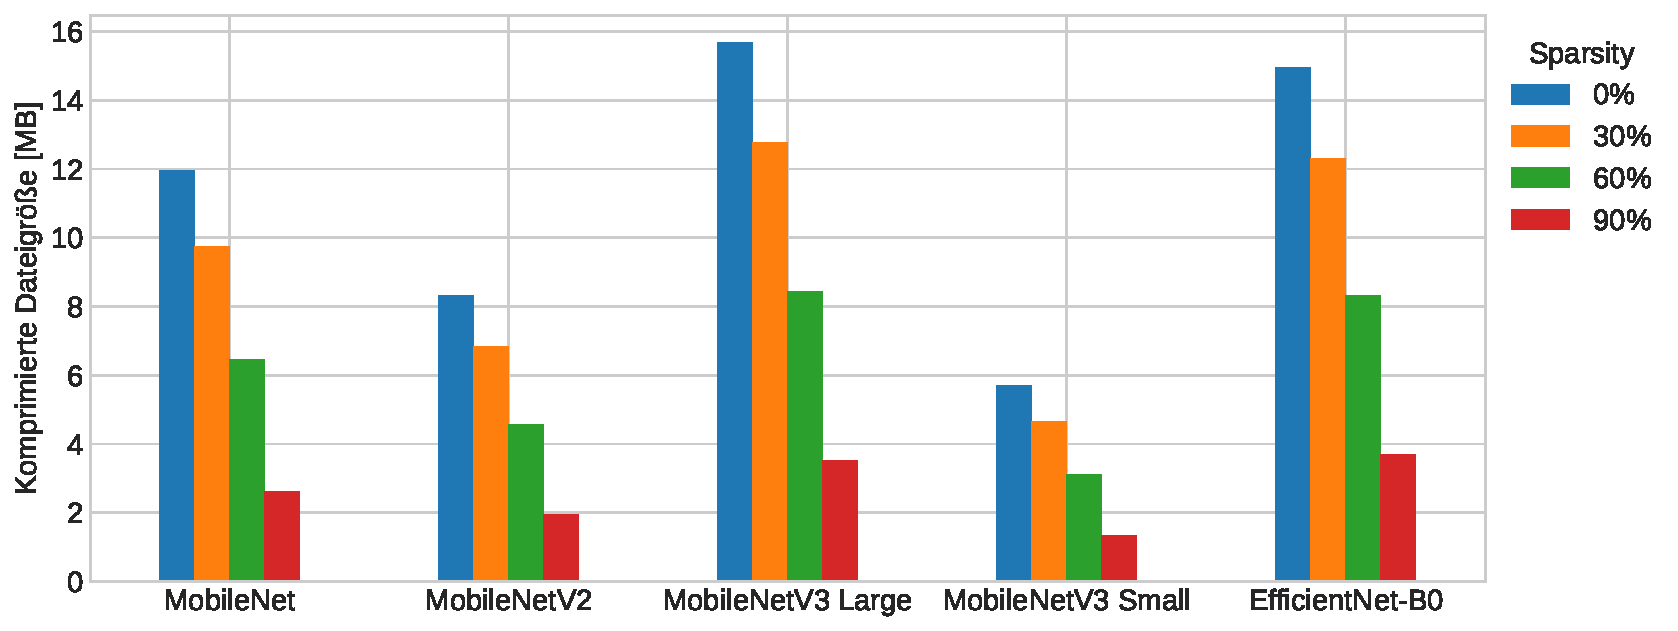
\includegraphics[width=\textwidth]{content/images/pruned_and_compressed.pdf}}
\caption{Dateigröße für Modelle mit $0\%$, $30\%$, $60\%$ und $90\%$ Sparsity nach Anwendung eines Kompressionsalgorithmus (gzip).}
\label{f4.3}
\end{figure}

Wie in Abbildung \ref{f4.3} gut zu ersehen ist, werden mit steigender Sparsity die komprimierten Modelle deutlich kleiner. So ist beispielsweise das MobileNet, welches ungepruned und komprimiert 12MB Hintergrundspeicher benötigt, nach Anwendung von Pruning mit einer gewünschten Sparsity von $90\%$ und Kompression nur noch 2.6MB groß. Die Speicherersparnis durch Kompression mit beispielsweise gzip hat den entscheidenden Nachteil, dass auf den komprimierten Modellen keine Inferenzen ausgeführt werden können. Um das Modell zu verwenden, muss die Kompression rückgängig gemacht werden und der volle Hintergrund- und Hauptspeicher für das Modell ohne Kompression wird benötigt. Jedoch ist in dem Fall, dass die Zielplattform, auf der die Inferenzen durchgeführt werden sollen, beispielsweise ein eingebettetes/verteiltes System ist, kann die Kombination aus Pruning und Kompression von entscheidendem Nutzen sein. Zum einen, wenn regelmäßig (z.B. als Update) trainierte Modelle über das Internet an eine entfernte Zielplattform gesendet werden sollen, oder aber auf der Zielplattform mit begrenzten Hintergrundspeicher sollen mehrere Modelle gespeichert werden, die aber nicht gleichzeitig verwendet werden. In diesen Fällen ist eine möglichst komprimierte Darstellung der Modelle hilfreich.


\subsection{Pruning und Quantisierung}
Bisher wurde betrachtet, was bei der Quantisierung und dem Pruning der vorgestellten Architekturen passiert. In diesem Abschnitt wird betrachtet, was passiert, wenn auf die vortrainierten Modelle als Erstes ein Pruning und anschließend eine Quantisierung angewendet wird.

Als Erstes ist in Abbildung \ref{f4.4} die Top-1 Genauigkeit der verschiedenen Modelle nach Anwendung von Pruning und Quantisierung dargestellt. Die ersten zwei Architekturen, die in dieser Grafik herausstechen, sind das MobileNetV3 Large und das EfficientNet-B0. Beim MobileNetV3 Large ist bei $0\%$ Sparsity erneut die schlechte Accuracy zu sehen, welche bereits in Abschnitt \ref{eval_quantisierung} diskutiert wurde. Durch das erneute Training während des Prunings hat sich die Genauigkeit des MobileNetV3 Large bei der Anwendung von Quantisierung verbessert. Zusätzlich fällt beim EfficientNet-B0 der Einbruch der Top-1 Accuracy beim Pruning mit einer gewünschten Sparsity von $30\%$ und anschließender Anwendung von Quantisierung auf. Dieser Einbruch der Genauigkeit hat sich beim Pruning auf eine gewünschte Sparsity von $60\%$ aber wieder ausgeglichen. Diese Ausreißer können möglicherweise durch ungünstig gewählte Parameter (Learning Rate Schedule, Pruning Schedule, Epochen, Batch Size, etc.) beim Training und Pruning der Architekturen entstehen. Am meisten profitieren die Architekturen MobileNet und MobileNetV2 von der Kombination aus Pruning und Quantisierung. Von beiden Architekturen ist die Top-1 Accuracy leicht besser, als wenn nur ein Pruning angewendet wird (siehe Abbildung \ref{f4.2}). Die restlichen Architekturen verhalten sich bezüglich der Top-1 Accuracy leicht schlechter als beim reinen Pruning ohne Anwendung von Quantisierung.

\begin{figure}[htbp]
\centerline{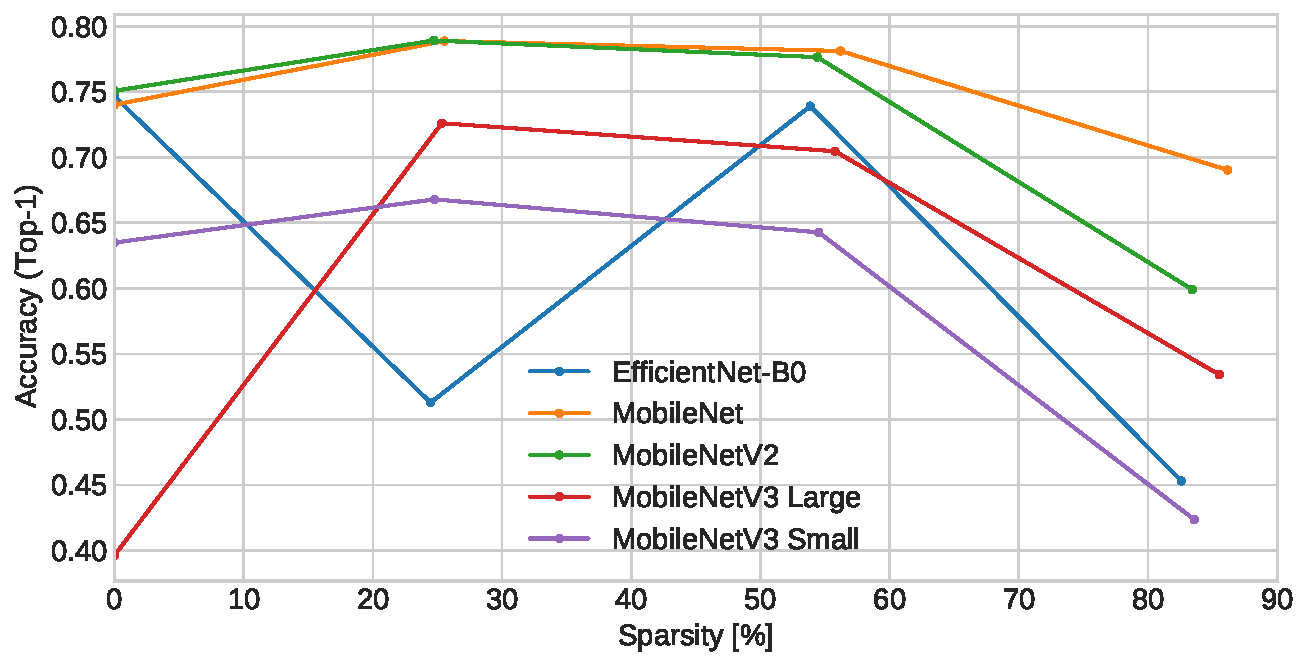
\includegraphics[width=0.8\textwidth]{content/images/sparsity_vs_accuracy_quantized.pdf}}
\caption{Genauigkeiten (Top-1) auf den Testdaten für die tatsächlichen Sparsity-Werte beim Pruning auf 0\% (ungepruned), 30\%, 60\% und 90\% Sparsity nach Anwendung von Quantisierung.}
\label{f4.4}
\end{figure}

Die Metriken Hintergrundspeicherbedarf, Hauptspeicherbedarf und Inferenzzeit sind für alle möglichen Sparsity Werte nahezu identisch und entsprechen den Werten für die quantisierten Modelle mit $0\%$ Sparsity in Tabelle \ref{t4.3}. Der Grund dafür wurde bereits in Abschnitt \ref{eval_pruning} diskutiert.

Besonders interessant wird die Kombination aus Pruning und Quantisierung, wenn diese Kombination nochmal mit einem Kompressionsalgorithmus wie gzip kombiniert wird. In Abschnitt \ref{eval_pruning} wurde bereits gezeigt, dass sich allein durch die Kombination von Pruning und einem Kompressionsalgorithmus die Größe der Modelle deutlich reduzieren lässt. Werden nun die geprunten Modelle vor der Kompression mit gzip noch quantisiert, dann ergeben sich für die einzelnen Architekturen die in Abbildung \ref{f4.5} dargestellten Dateigrößen.

\begin{figure}[htbp]
\centerline{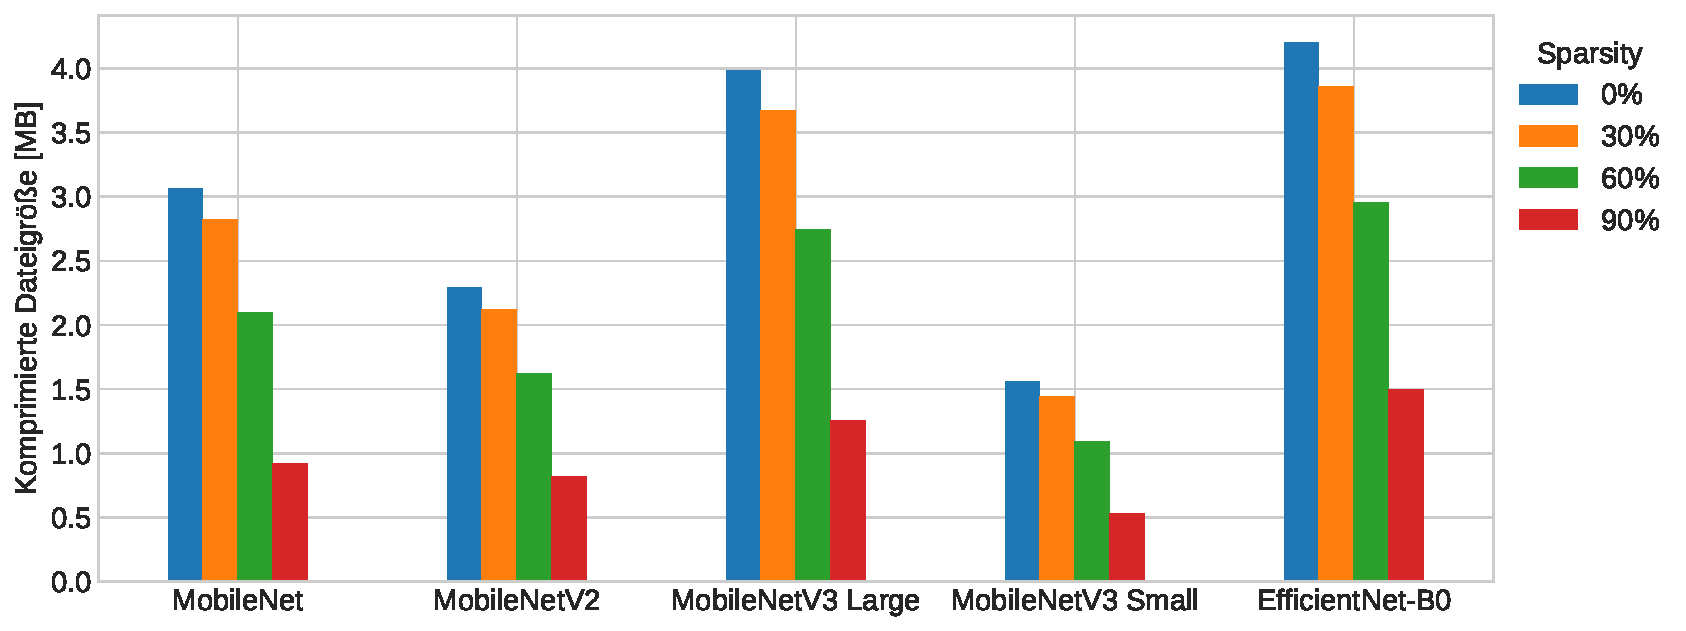
\includegraphics[width=\textwidth]{content/images/pruned_and_compressed_quantized.pdf}}
\caption{Dateigröße für Modelle mit $0\%$, $30\%$, $60\%$ und $90\%$ Sparsity nach Anwendung von Quantisierung und eines Kompressionsalgorithmus (gzip).}
\label{f4.5}
\end{figure}

Verglichen mit den Dateigrößen in Abbildung \ref{f4.3} hat die Quantisierung der Modelle vor der Kompression die Dateigröße nochmal deutlich reduziert. Beispielsweise hat das MobileNet nach der Anwendung von Pruning ($90\%$ Sparsity), Quantisierung und Kompression mittels gzip nur noch einen Hintergrundspeicherbedarf von 0.9MB. Verglichen mit dem komprimierten MobileNet ohne Anwendung von Pruning und Quantisierung mit 12MB Hintergrundspeicherbedarf ist das eine Reduktion um das 13-fache.

Das kleinste Modell nach Anwendung von Pruning ($90\%$ Sparsity), Quantisierung und Kompression ist das MobileNetV3 Small mit 0.5MB Hintergrundspeicherbedarf.


\section{Einfluss der Optimierungen auf die Klassen}
Der folgende Abschnitt stellt eine weitere Evaluationsmetrik vor, welche angelehnt ist an das Paper "What Do Compressed Deep Neural Networks Forget?" von Sara Hooker et al. \cite{hooker_what_2020}.

Um die Architekturen untereinander zu vergleichen und die Auswirkungen von Quantisierung und Pruning auf die vorgestellten Architekturen zu bewerten, wurden in dieser Arbeit bisher unter anderem die Top-1 und Top-3 Genauigkeit verwendet. Diese Top-1 und Top-3 Genauigkeit gibt das Verhältnis zwischen der Anzahl der korrekt klassifizierten Beispiele zu der Anzahl aller Beispiele an. Bisher wurde in dieser Arbeit diese Genauigkeit unabhängig von der Klassenzugehörigkeit der jeweiligen Beispiele bestimmt. Jedoch lässt sich die Genauigkeit auch für jede einzelne Klasse bestimmen, indem die Anzahl der korrekt klassifizierten Beispiele einer Klasse zu der Anzahl aller Beispiele einer Klasse für alle Klassen ins Verhältnis gesetzt wird. Wird angenommen, dass sich der Verlust durch die Optimierungstechniken gleichmäßig auf die Genauigkeit der einzelnen Klassen auswirkt, dann würde sich das Modell nach Anwendung der Optimierungen noch annähernd gleich verhalten. Es wurde jedoch gezeigt, dass Pruning und Quantisierung die Genauigkeit der einzelnen Klassen eines Modells unterschiedlich stark beeinflussen \cite{hooker_what_2020}. Dies kann beispielsweise zur Folge haben, dass eine Klasse durch die Anwendung von Pruning deutlich an Genauigkeit verliert, während die anderen Klassen nur leicht an Genauigkeit verlieren. Der ungleichmäßige Genauigkeitsverlust kann in einigen Anwendungsbereichen, wie bei selbstfahrenden Autos oder in der Medizintechnik, katastrophale Folgen haben. Aus diesem Grund sollte nicht allein auf die generelle Genauigkeit vertraut werden, sondern auch für jede Klasse separat die Genauigkeit betrachtet werden. 

\begin{table}[ht]
\centering
\begin{tabular}{l|llll|llll}
\toprule
               & \multicolumn{4}{c}{MobileNet}           & \multicolumn{4}{c}{EfficientNet-B0} \\
               &       0\% &   30\% &   60\% &    Quant. &    0\% &   30\% &   60\%   & Quant. \\
\midrule
Automobil      &     0.738 &  0.862 &  0.844 &     0.732 &    0.792 &  0.870 &  0.873 &     0.771 \\
Flugzeug       &     0.697 &  0.835 &  0.836 &     0.689 &    0.847 &  0.817 &  0.789 &     0.817 \\
Frosch         &     0.786 &  0.845 &  0.830 &     0.806 &    0.825 &  0.835 &  0.818 &     0.824 \\
Hirsch         &     0.724 &  0.764 &  0.755 &     0.715 &    0.785 &  0.752 &  0.717 &     0.780 \\
Hund           &     0.665 &  0.642 &  0.620 &     0.666 &    0.575 &  0.601 &  0.580 &     0.552 \\
Katze          &     0.441 &  0.602 &  0.627 &     0.416 &    0.521 &  0.655 &  0.628 &     0.542 \\
LKW &     0.917 &  0.861 &  0.849 &     0.922 &    0.894 &  0.854 &  0.829 &     0.895 \\
Pferd          &     0.761 &  0.838 &  0.820 &     0.768 &    0.844 &  0.802 &  0.776 &     0.833 \\
Schiff         &     0.841 &  0.860 &  0.860 &     0.844 &    0.898 &  0.879 &  0.855 &     0.886 \\
Vogel          &     0.707 &  0.679 &  0.654 &     0.690 &    0.533 &  0.705 &  0.675 &     0.447 \\
\bottomrule
\end{tabular}
\caption{Klassenweise Top-1 Accuracy der MobileNet und EfficientNet-B0 Architekturen auf dem CIFAR-10 Datensatz für die Modelle mit $0\%$, $30\%$, $60\%$ und $90\%$ Sparsity und dem ungeprunten quantisierten Modellen (Quant.).}
\label{t4.6}
\end{table}

Im Folgenden wird exemplarisch an der MobileNet und EfficientNet-B0 Architektur betrachtet, wie sich ein Pruning mit $30\%$, $60\%$ und $90\%$ Sparsity und eine Quantisierung der ungeprunten Modelle auf die einzelnen Klassen auswirkt. Dazu sind in Tabelle \ref{t4.6} die Top-1 Genauigkeiten auf den Testdaten für jede der 10 Klassen des CIFAR-10 Datensatzes dargestellt. Was in der Tabelle \ref{t4.6} direkt auffällt ist, dass die Genauigkeiten jeder Klasse sehr unterschiedlich sein können. Beispielsweise ist beim nicht geprunten MobileNet die Genauigkeit für die Klasse Katze $44.1\%$ während die Klasse LKW eine Genauigkeit von $91.7\%$ besitzt. Damit scheint das in dieser Arbeit trainierte MobileNet besser dazu in der Lage zu sein LKWs zu klassifizieren als Katzen.

Um nun zu visualisieren, wie sich die Genauigkeit der einzelnen Modelle während des Prunings und der Quantisierung im Vergleich zum Ausgangsmodell mit $0\%$ Sparsity verändert hat, wurde für jede Klasse die Differenz zwischen dem optimierten Modell und dem Ausgangsmodell gebildet.

Abbildung \ref{f4.6} zeigt die Veränderung der Genauigkeit in Prozentpunkten für die MobileNet Architektur beim Pruning mit den verschiedenen gewünschten Sparsity-Werten. Würde sich die Veränderung der Genauigkeit durch die Anwendung von Pruning gleichermaßen auf alle Klassen auswirken, müssten alle Balken in dem Balkendiagramm die gleiche Länge und Ausrichtung haben. Jedoch ist sehr gut ersichtlich, wie unterschiedlich die Veränderung durch das Pruning ist. Beispielsweise hat sich während des Prunings auf $30\%$ Sparsity die Klasse Katze um $16.1\%$-Punkte verbessert, während sich die Klasse LKW um $5.6\%$-Punkte verschlechtert hat. Wird das MobileNet auf $90\%$ Sparsity gepruned lässt sich gut erkennen, wie die Klasse Vogel um $19.8\%$-Punkte Genauigkeit verliert. Das ist ein gutes Beispiel dafür, dass es wichtig ist die Genauigkeiten der einzelnen Klassen im Blick zu haben, da die MobileNet Architektur beim Pruning auf $90\%$ Sparsity lediglich $6\%$-Punkte an Genauigkeit verloren hat (siehe Abschnitt \ref{eval_pruning}), jedoch hat die Klasse Vogel $19.8\%$-Punkte Genauigkeit eingebüßt. Wenn die Anwendung aber Wert darauf legt, dass Vögel korrekt klassifiziert werden, kann die Betrachtung der generellen Top-1 Accuracy über alle Klassen täuschen.

\begin{figure}[htbp]
\centerline{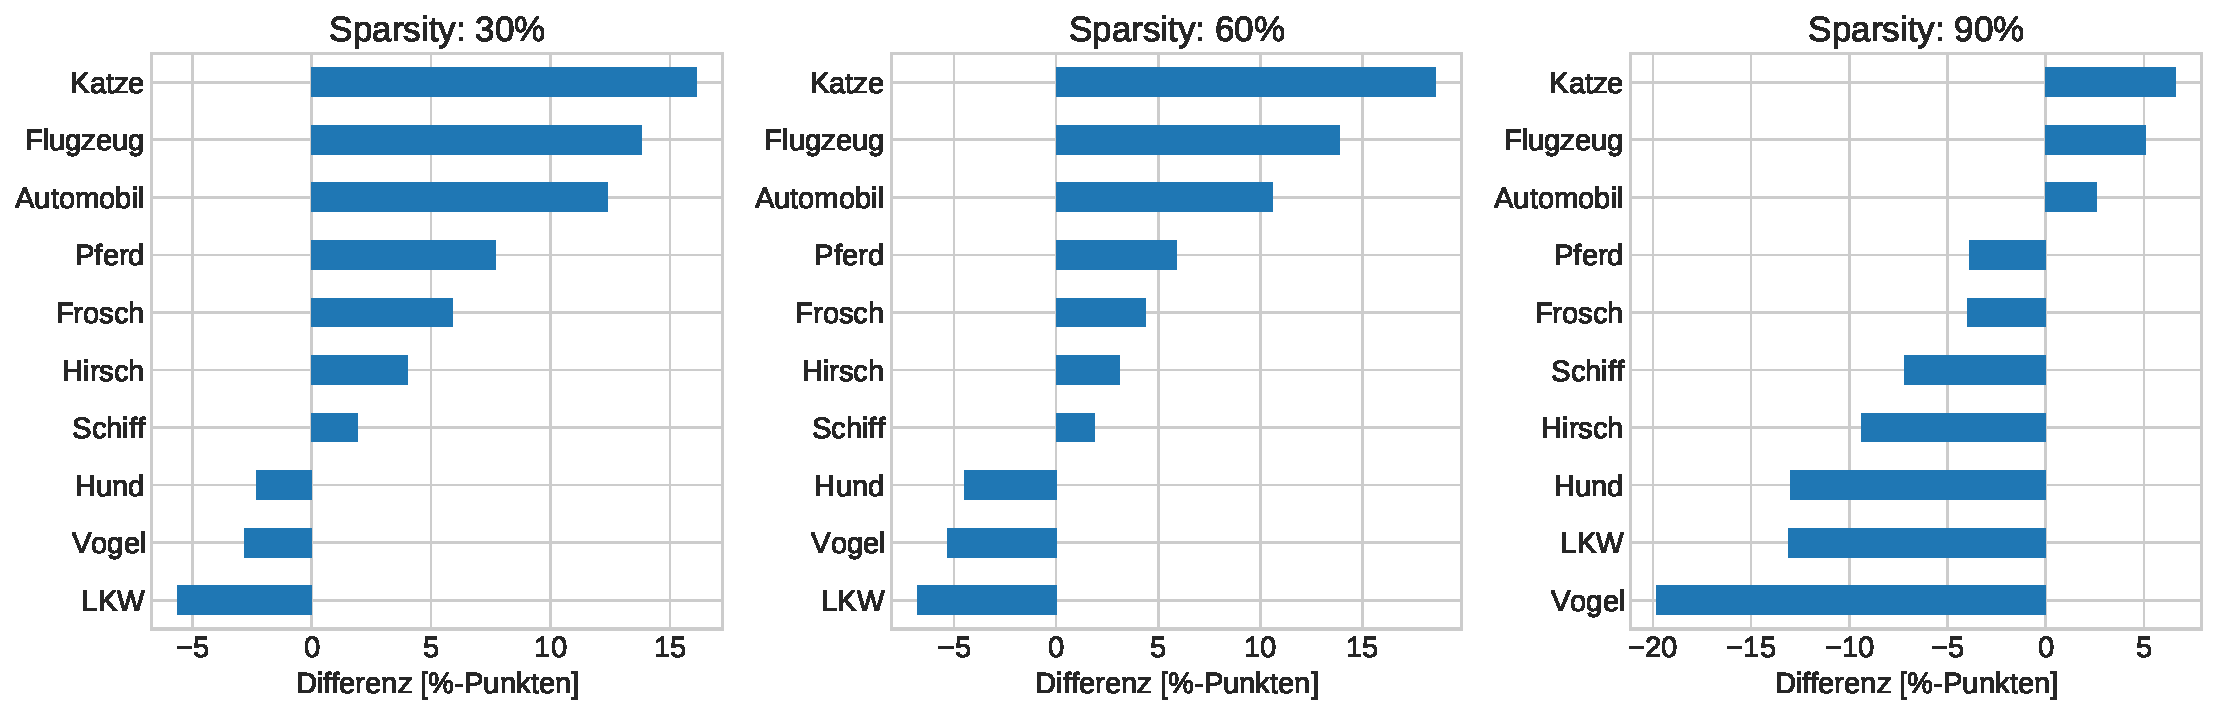
\includegraphics[width=\textwidth]{content/images/classwise_acc_change_pruning_mobilenet.pdf}}
\caption{Veränderung der klassenweisen Top-1 Genauigkeit der geprunten MobileNet Modelle mit $30\%$, $60\%$ und $90\%$ Sparsity in Prozentpunkten.}
\label{f4.6}
\end{figure}

In Abbildung \ref{f4.7} ist die klassenweise Veränderung der EfficientNet-B0 Architektur für die verschiedenen Sparsity-Werte dargestellt. Wie auch hier zu sehen ist, beeinflusst das Pruning die Genauigkeit der einzelnen Klassen sehr unterschiedlich. Am meisten profitieren die Klassen Vogel, Katze und Automobil vom Pruning der EfficientNet-B0 Architektur. Wie in Abbildung \ref{f4.2} ersichtlich, verliert die EfficientNet-B0 Architektur im Verlauf des Prunings auf $90\%$ gewünschte Sparsity insgesamt $14\%$-Punkte an Top-1 Genauigkeit. Das ist deutlich mehr Verlust als beim MobileNet während des Prunings. Dies spiegelt sich auch in der klassenweisen Genauigkeit in Abbildung \ref{f4.7} wieder. Bei $90\%$ Sparsity haben alle Klassen an Genauigkeit verloren. Die Klassen LKW, Flugzeug und Hirsch haben dabei mit über $20\%$-Punkten den größten Verlust an Top-1 Genauigkeit.

\begin{figure}[htbp]
\centerline{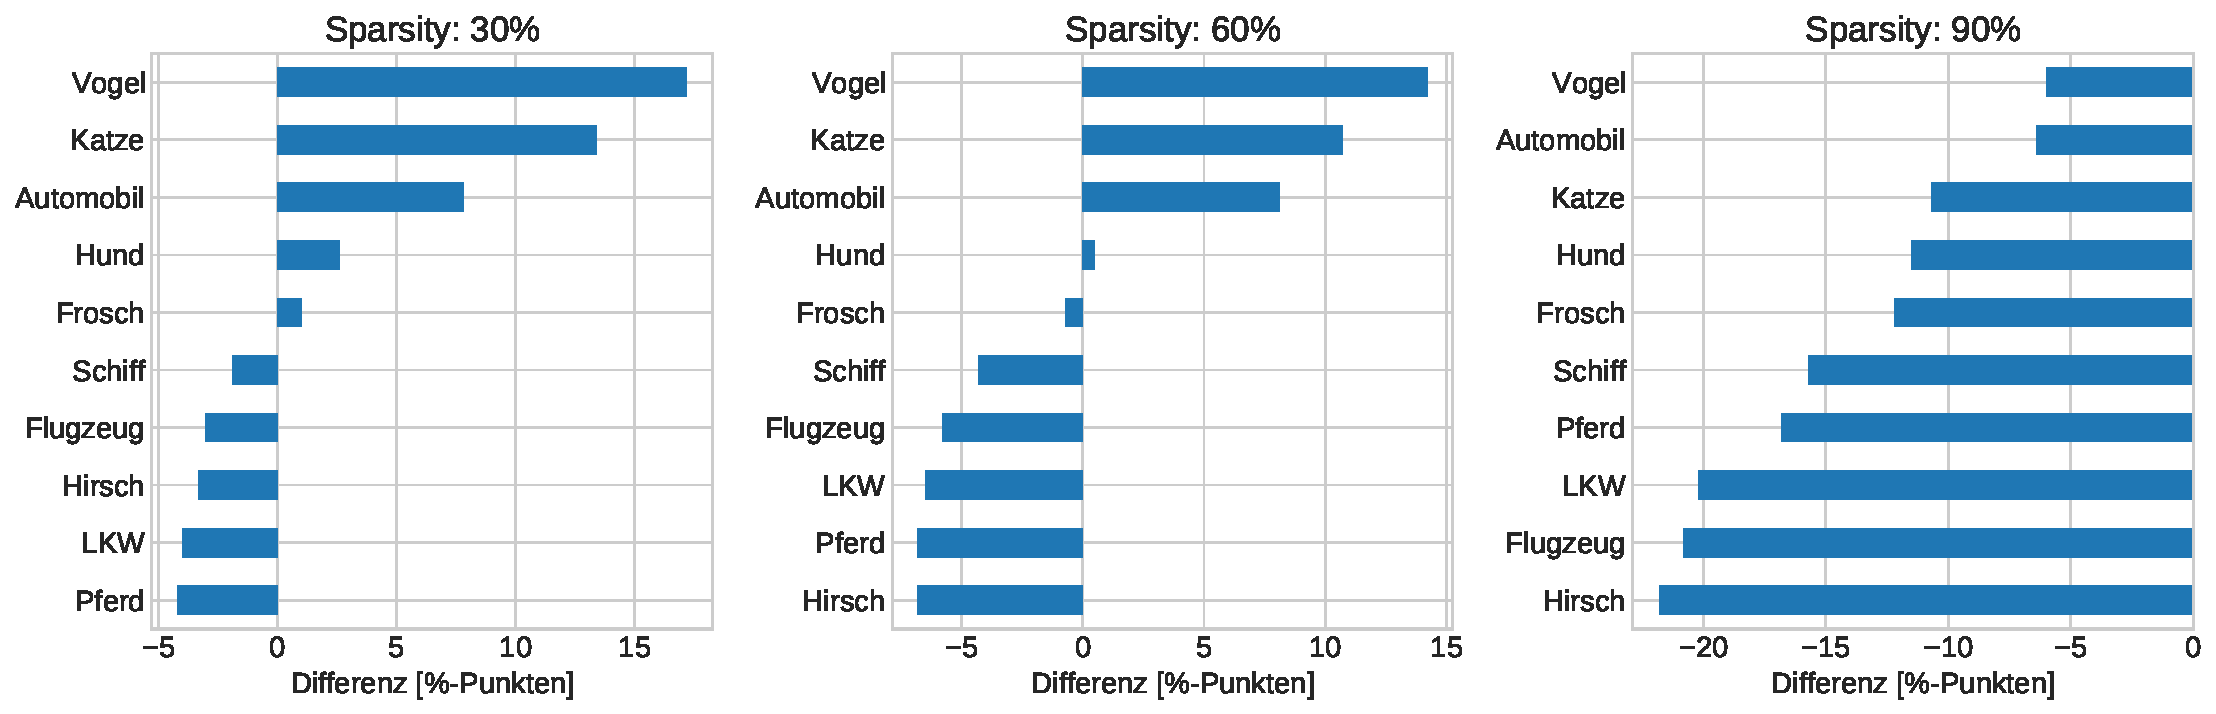
\includegraphics[width=\textwidth]{content/images/classwise_acc_change_pruning_efficientnet-b0.pdf}}
\caption{Veränderung der klassenweisen Top-1 Genauigkeit der geprunten EfficientNet-B0 Modelle mit $30\%$, $60\%$ und $90\%$ Sparsity in Prozentpunkten.}
\label{f4.7}
\end{figure}

Nachdem nun der klassenweise Verlust bei der Anwendung von Pruning auf die zwei exemplarischen Architekturen MobileNet und EfficientNet-B0 diskutiert wurde, stellt sich noch die Frage, wie sich die Post-Training Quantisierung auf die Genauigkeit der einzelnen Klassen auswirkt. Dazu stellt Abbildung \ref{f4.8} die Veränderungen der klassenweisen Top-1 Genauigkeiten der MobileNet und EfficientNet-B0 Architekturen dar.

\begin{figure}[htbp]
\centerline{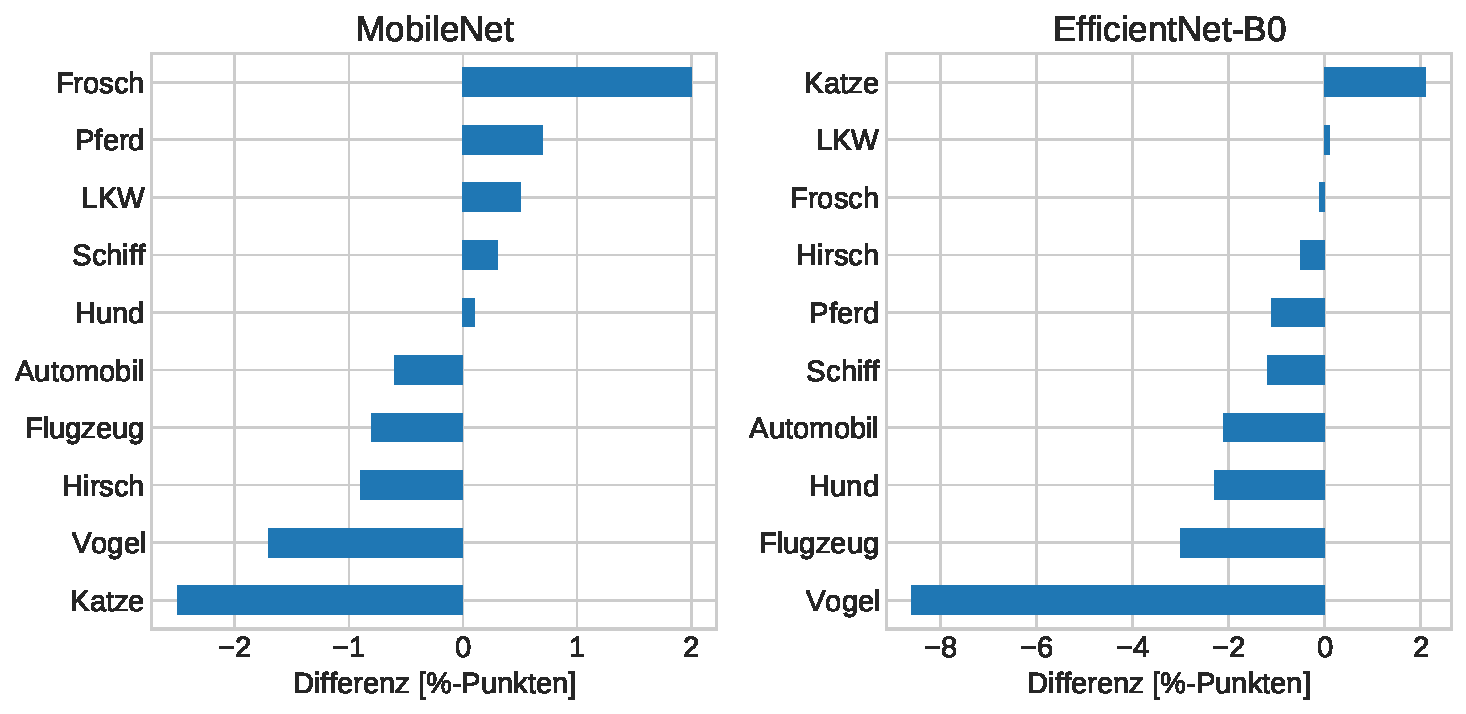
\includegraphics[width=0.7\textwidth]{content/images/classwise_acc_change_quantization.pdf}}
\caption{Differenz der klassenweisen Top-1 Accuracy des nicht quantisierten MobileNet Modells und des quantisierten MobileNet Modells.}
\label{f4.8}
\end{figure}

Genau wie beim Pruning ist bei der Quantisierung ebenfalls deutlich zu erkennen, dass die Anwendung dieser Optimierungstechnik zu einer ungleichmäßigen Veränderung der Genauigkeiten der einzelnen Klassen geführt hat. Am wenigsten hat die Quantisierung die Genauigkeiten der einzelnen Klassen bei der MobileNet Architektur beeinflusst. Bei dieser Architektur hat die Klasse Frosch mit $2\%$-Punkten verbesserter Genauigkeit am stärksten von der Quantisierung profitiert. Die Klasse Katze hat mit $2.5\%$-Punkten den größten Verlust durch die Quantisierung zu verzeichnen. Bei der EfficientNet-B0 Architektur wurde die Genauigkeit der einzelnen Klassen deutlich stärker von der Quantisierung beeinflusst als beim MobileNet. Beim EfficientNet-B0 profitiert die Klasse Katze mit $2.1\%$-Punkte von der Quantisierung am meisten. Die Klasse Vogel ist beim quantisierten EfficientNet-B0 erneut ein gutes Beispiel dafür, warum die Betrachtung der klassenweisen Genauigkeit besonders wichtig ist. Die Klasse Vogel hat beim Quantisieren der Architektur $8.6\%$-Punkte an Genauigkeit verloren, während der Verlust an Genauigkeit der anderen Klassen recht begrenzt ist. Angenommen die Klasse Vogel ist für den Anwendungsbereich, in der das Modell eingesetzt werden soll, von besonderer Bedeutung, kann dieser enorme Genauigkeitsverlust zu Problemen führen. Insgesamt verliert die EfficientNet-B0 Architektur durch die Anwendung von Quantisierung nur $0.5\%$-Punkte an Top-1 Genauigkeit (siehe Abschnitt \ref{eval_training} und Abschnitt \ref{eval_quantisierung}). Daran lässt sich gut erkennen, dass die generelle Genauigkeit über alle Klassen wichtige Veränderungen für einzelne Klassen verschleiert.



\section{Optimierungen}
Bisher wurden in dieser Arbeit ausschließlich die unveränderten Standardvarianten der Architekturen MobileNet, MobileNetV2, MobileNetV3 und EfficientNet vorgestellt und untersucht. Diese Architekturen haben sich zum Ziel gesetzt, besonders wenig Ressourcen zu benötigen, um in einem mobilen oder eingebetteten System Anwendung zu finden. Durch Optimierungstechniken wie Quantisierung und Pruning lässt sich der Ressourcenbedarf dieser Architekturen drastisch reduzieren (siehe Abschnitt \ref{ergebnisse}). Dies geht aber oft auf Kosten einer verminderten Genauigkeit der trainierten und optimierten Modelle. Zusätzlich werden in den vorgestellten Architekturen teilweise Schichten verwendet, die noch nicht so gut von Hardware oder Software unterstützt werden. Dies kann beispielsweise zu einer erhöhten Inferenzzeit führen. In diesem Abschnitt soll untersucht und diskutiert werden, was für Optimierungen durchgeführt werden können, um die vorgestellten Architekturen weiter zu optimieren.

Bereits im Abschnitt \ref{eval_training} wurde diskutiert, dass der exzessive Gebrauch von Squeeze-And-Excitation Modulen zu einer erhöhten Inferenzzeit auf dem Raspberry Pi 4 führt. Dies ist vermutlich auch der Grund dafür, warum die EfficientNet-B0 Architektur eine um $54.7\%$ erhöhte Inferenzzeit im Vergleich zu der ähnlich großen MobileNetV3 Large Architektur besitzt. Die EfficientNet-B0 Architektur ist architekturell recht ähnlich zu der MobileNetV3 Large Architektur, jedoch verwendet sie $50\%$ mehr Squeeze-And-Excitation Module als die MobileNetV3 Large Architektur.

Um mitunter das Problem mit den Squeeze-And-Excitation Modulen zu beheben, wurden die in Abschnitt \ref{efficientnet} beschriebenen EfficientNet-lite Architekturen veröffentlicht \cite{liu_higher_2020}. Diese EfficientNet-lite Architekturen haben eine Reihe an architekturellen Optimierungen vorgenommen, welche eine breitere Hardwarekompatibilität, weniger Parameter und bessere Quantisierbarkeit erreichen sollen. Die vorgenommenen Optimierungen sind \cite{liu_higher_2020}:
\begin{itemize}
\item Squeeze-And-Excitation Module wurden entfernt, um eine bessere und breitere Hardwarekompatibilität zu ermöglichen.
\item Die Swish Aktivierungsfunktion wurde durch die ReLU6 Aktivierungsfunktion ersetzt, um eine bessere Quantisierbarkeit mittels Post-Training Quantization zu erreichen.
\item Um die Größe der Architektur und die Anzahl an Berechnungen zu verringern, wurden einige Parameter vom Compound Scaling ausgeschlossen.
\end{itemize}
Das Problem mit diesen EfficientNet-lite Architekturen ist, dass zum Zeitpunkt, zu dem diese Arbeit entstanden ist, noch kein Paper zu diesen Architekturen veröffentlicht wurde. Es existierte lediglich ein Blog-Post von TensorFlow, welcher grob die Optimierungen dieser Architekturen beschreibt \cite{liu_higher_2020}. Von TensorFlow gibt es zwar auf dem ImageNet Datensatz vortrainierte EfficientNet-lite Modelle \footnote{\url{https://tfhub.dev/s?q=EfficientNet-Lite}}, jedoch ist es nicht gelungen das in dieser Arbeit verwendete Evaluationsverfahren auf diese Architekturen anzuwenden. 

Eine weitere Architektur, zu der eine optimierte Variante existiert, ist die MobileNetV3 Large/Small Architektur. TensorFlow bietet für diese beiden Architekturen jeweils eine so genannte Minimalistic-Variante \footnote{\url{https://www.tensorflow.org/api_docs/python/tf/keras/applications/MobileNetV3Large}} \footnote{\url{https://www.tensorflow.org/api_docs/python/tf/keras/applications/MobileNetV3Small}} an, welche teilweise recht ähnliche Optimierungen vornimmt wie die EfficientNet-lite Architekturen. Diese Optimierungen sind:
\begin{itemize}
\item Ebenfalls wie bei den EfficientNet-lite Architekturen wurden die Squeeze-And-Excitation Module entfernt.
\item Die Hard-Swish Aktivierungsfunktion wurde durch die ReLU Aktivierungsfunktion ersetzt.
\item Außerdem wurden Convolutions mit einer Kernelgröße von $5 \times 5$ durch Convolutions mit einer Kernelgröße von $3 \times 3$ ausgetauscht.
\end{itemize}
Ansonsten entsprechen die MobileNetV3 Minimalistic Architekturen vom Aufbau den normalen MobileNetV3 Architekturen. Zusätzlich sind die MobileNetV3 Minimalistic Architekturen sehr gut in der TensorFlow Bibliothek implementiert und lassen sich genauso wie die anderen vorgestellten Architekturen verwenden.

Im Folgenden wird anhand der MobileNetV3 Minimalistic Architekturen untersucht, inwieweit sich die architekturellen Optimierungen auf die MobileNetV3 Architektur auswirken und wie sich die MobileNetV3 Minimalistic Architekturen unter Anwendung von Quantisierung und Pruning verhalten.

Dazu werden die MobileNetV3 Large/Small Minimalistic Architekturen zuerst auf dem CIFAR-10 Datensatz trainiert und anschließend analog zu den anderen Architekturen evaluiert. Bei dem Training und beim Pruning musste von dem einheitlichen Setup für alle Experimente (siehe Abschnitt \ref{training} und Abschnitt \ref{impl_pruning}) leicht abgewichen werden. Das bedeutet, dass die initiale und schlussendliche Learning Rate beim Training und Pruning um den Faktor $10^{-1}$ reduziert wurde. Der Grund dafür ist, dass ansonsten der Loss der MobileNetV3 Minimalistic Architekturen während des Trainings dazu tendiert zu divergieren. Nach dem Training der MobileNetV3 Minimalistic Architekturen ergeben sich folgende Kennwerte, welche in Tabelle \ref{t4.7} dargestellt sind.

\begin{table}[ht]
\centering
\begin{tabular}{lllllll}
\toprule
 & Parameter &  Top-1 &  Top-3 &  Datei [MB] &  RAM [MB] &  Inferenz [µs] \\
\midrule
            Large &  2.7 Mio. & 0.6949 & 0.9128 &     10.6120 &   14.2344 &        5297 \\
            Small &  1.0 Mio. & 0.6099 & 0.8755 &      4.1234 &    6.1797 &        1826 \\
\bottomrule
\end{tabular}
\caption{Kennwerte der MobileNetV3 Large/Small Minimalistic Modelle nach dem Training auf dem CIFAR-10 Datensatz. Top-1/Top-3 entsprechen der Top-1/Top-3 Genauigkeit auf den Testdaten.}
\label{t4.7}
\end{table}

Wird die Tabelle \ref{t4.7} mit der Tabelle \ref{t4.1} und Tabelle \ref{t4.2} verglichen, fällt zum einen auf, dass die Parameterzahl der MobileNetV3 Minimalistic Modelle um einiges geringer ist als bei den normalen MobileNetV3 Architekturen. Dies ergibt sich daraus, dass die Squeeze-And-Excitation Module entfernt wurden und die $5 \times 5$ Convolutions durch $3 \times 3$ Convolutions ersetzt wurden. Dies sorgt beides für eine verringerte Parameterzahl der Architekturen. Zum anderen fällt auf, dass die Inferenzzeit beider Minimalistic Architekturen gesunken ist. Dies ist vermutlich bedingt durch die verringerte Parameterzahl und durch das Entfernen der schlecht unterstützten Squeeze-And-Excitation Module. Weiter kann man in Tabelle \ref{t4.7} erkennen, dass die Genauigkeit des MobileNetV3 Large Minimalistic nahezu gleich geblieben ist zu der Genauigkeit des normalen MobileNetV3 Large. Das MobileNetV3 Small Minimalistic hat leicht an Genauigkeit verloren. Die Dateigröße der Modelle und der Bedarf an Hauptspeicher ist ebenfalls stark gesunken, was durch die gesunkene Parameterzahl bedingt ist.

Werden nun diese Modelle mittels Post-Training Float-Fallback Quantisierung quantisiert, ergeben sich die in Tabelle \ref{t4.8} beschriebenen Kennwerte für die Modelle. In dieser Tabelle lässt sich gut erkennen, dass sich durch die Quantisierung die Größe und Inferenzzeit der Modelle drastisch reduziert hat. Nach der Quantisierung benötigt das MobileNetV3 Small Minimalistic auf dem Raspberry Pi 4 nur noch 1.1ms für die Inferenz eines Eingabebildes.

\begin{table}[ht]
\centering
\begin{tabular}{lllllll}
\toprule
 & Parameter &  Top-1 &  Top-3 &  Datei [MB] &  RAM [MB] &  Inferenz [µs] \\
\midrule
            Large &  2.7 Mio. & 0.7050 & 0.9269 &      3.1612 &   5.57420 &        2839 \\
            Small &  1.0 Mio. & 0.6343 & 0.8879 &      1.3065 &   4.37891 &        1118 \\
\bottomrule
\end{tabular}
\caption{Kennwerte der trainierten und quantisierten MobileNetV3 Large/Small Minimalistic Modelle.}
\label{t4.8}
\end{table}

Um die Veränderung durch die Quantisierung im Verhältnis zu den nicht quantisierten Modellen besser zu visualisieren, wird in Abbildung \ref{f4.9} genau wie in Abschnitt \ref{eval_quantisierung} die prozentuale Veränderung der einzelnen Metriken für jedes Modell in Bezug auf die nicht quantisierten Modelle dargestellt. Dabei werden zusätzlich neben den Minimalistic-Varianten der MobileNetV3 Architektur auch die quantisierten MobileNetV3 Large/Small Architekturen dargestellt.

\begin{figure}[htbp]
\centerline{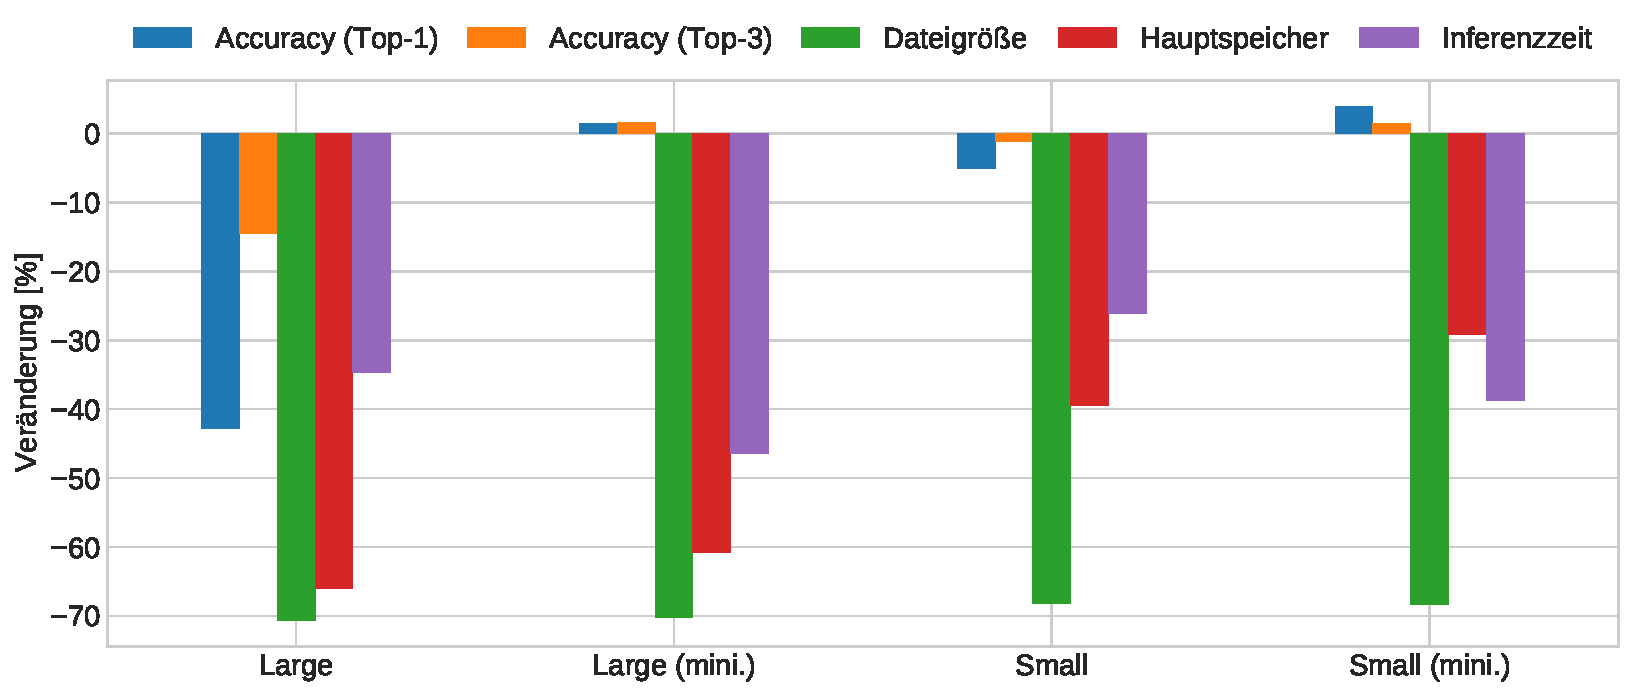
\includegraphics[width=0.9\textwidth]{content/images/quantization_improvements_mnv3mini.pdf}}
\caption{Prozentuale Veränderung der Metriken der MobileNetV3 Varianten durch Anwendung von Quantisierung.}
\label{f4.9}
\end{figure}

Die Abbildung \ref{f4.9} zeigt, wie die MobileNetV3 Minimalistic Architektur bei der Quantisierung durch die architekturellen Optimierungen profitiert. Während beide MobileNetV3 Architekturen durch die Quantisierung an Genauigkeit verlieren, gewinnen die beiden MobileNetV3 Minimalistic an Genauigkeit. Selbst das MobileNetV3 Large Minimalistic gewinnt leicht an Genauigkeit, obwohl sich das normale MobileNetV3 Large am stärksten von allen betrachteten Architekturen durch die Quantisierung verschlechtert hat. Zusätzlich fällt auf, dass sich bei allen Minimalistic-Varianten die Inferenzzeit durch die Quantisierung stärker hat reduzieren lassen als bei den normalen MobileNetV3 Architekturen. Dies kann möglicherweise mit den fehlenden Squeeze-And-Excitation Modulen zusammenhängen, welche auf dem Raspberry Pi 4 die Inferenzzeit deutlich verringert haben. Jedoch konnten die MobileNetV3 Minimalistic Architekturen den Bedarf an Hauptspeicher nicht so stark reduzieren wie die normalen MobileNetV3 Architekturen.

Werden nun die MobileNetV3 Architekturen gepruned und zusätzlich noch quantisiert, verändert sich die Genauigkeit mit zunehmender Sparsity wie in Abbildung \ref{f4.10} dargestellt.

\begin{figure}[htbp]
\centerline{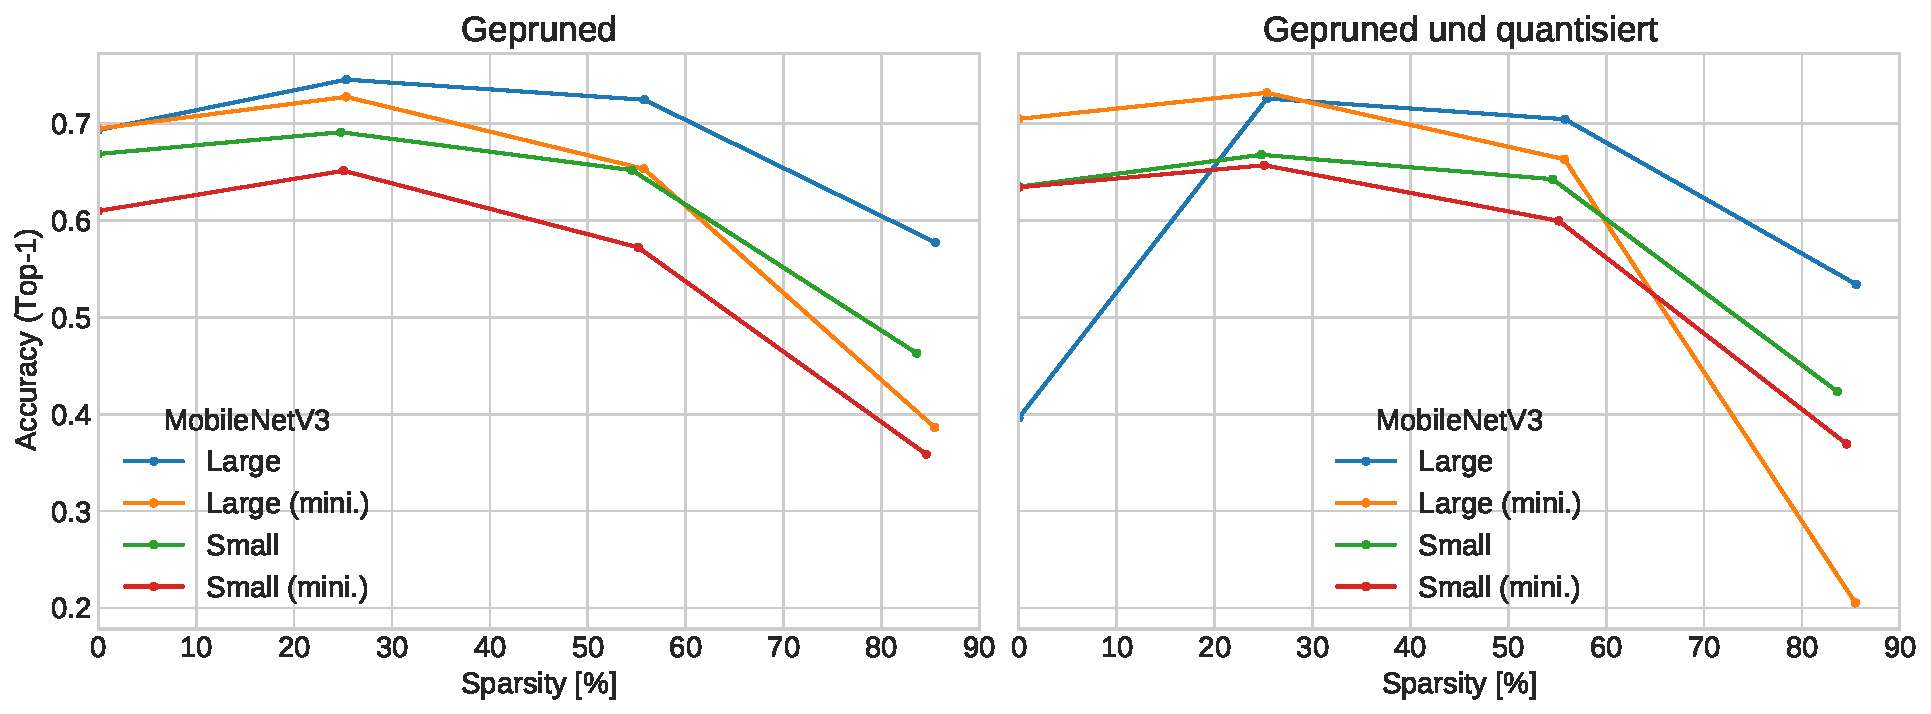
\includegraphics[width=\textwidth]{content/images/sparsity_vs_accuracy_mnv3mini.pdf}}
\caption{Genauigkeiten (Top-1) der MobileNetV3 Architekturen auf den Testdaten für die tatsächlichen Sparsity-Werte beim Pruning auf $0\%$ (ungepruned), $30\%$, $60\%$ und $90\%$ Sparsity und auf der linken Seite nach anschließender Post-Training Quantisierung dieser Modelle.}
\label{f4.10}
\end{figure}

Es lässt sich in Abschnitt \ref{eval_pruning} erkennen, dass auch die MobileNetV3 Minimalistic Modelle mit zunehmender Sparsity an Genauigkeit verlieren. Zusätzlich lässt sich erkennen, dass der Verlust an Genauigkeit bei den Minimalistic-Varianten mit zunehmender Sparsity etwas stärker ausfällt als bei den normalen MobileNetV3 Modellen. Bei dem quantisierten MobileNetV3 Large Minimalistic sinkt die Top-1 Genauigkeit auf den Testdaten sogar auf ca. $20\%$ ab, während das einfache MobileNetV3 Large beim Pruning auf $90\%$ Sparsity und anschließender Quantisierung eine Genauigkeit von $53\%$ beibehält. Der Grund dafür, warum die MobileNetV3 Minimalistic Architekturen bei zunehmender Sparsity schlechtere Genauigkeiten erzielen als die normalen MobileNetV3 Architekturen, ist vermutlich, dass die Minimalistic-Varianten von Grund auf schon weniger Parameter besitzen als die normalen MobileNetV3 Architekturen und dadurch stärker auf eine weitere Reduzierung der Parameter reagieren. Außer dem Genauigkeitsverlust ändern sich die anderen Metriken der MobileNetV3 Minimalistic Architekturen aber nicht, wie bereits in Abschnitt \ref{eval_pruning} diskutiert. Abgesehen von der Genauigkeit sind die anderen Metriken der MobileNetV3 Minimalistic Modelle in derselben Größenordnung wie in Tabelle \ref{t4.7} und Tabelle \ref{t4.8} beschrieben.

Werden nun aber die geprunten und geprunten \& quantisierten MobileNetV3 Minimalistic Modelle wie im Abschnitt \ref{eval_pruning} mittels des Kompressionsalgorithmus gzip komprimiert, lässt sich die Größe der einzelnen Architekturen nochmals deutlich reduzieren. Abbildung \ref{f4.11} zeigt die Dateigrößen der komprimierten MobileNetV3 Modelle inklusive der Minimalistic-Varianten für die verschiedenen Sparsity-Werte. Wie auch in Abschnitt \ref{eval_pruning} gesehen, lässt sich die Größe der einzelnen Architekturen mit zunehmender Sparsity immer weiter komprimieren. Damit ist die kleinste betrachtete Architektur in diesem Paper die MobileNetV3 Small Minimalistic Architektur mit ca. 1 Millionen Parametern und einer Dateigröße des nicht quantisierten Modells von 6.2MB. Wird dieses Modell komprimiert, quantisiert und auf $90\%$ Sparsity gepruned, beträgt die Dateigröße nur noch 0.36MB.

\begin{figure}[htbp]
\centerline{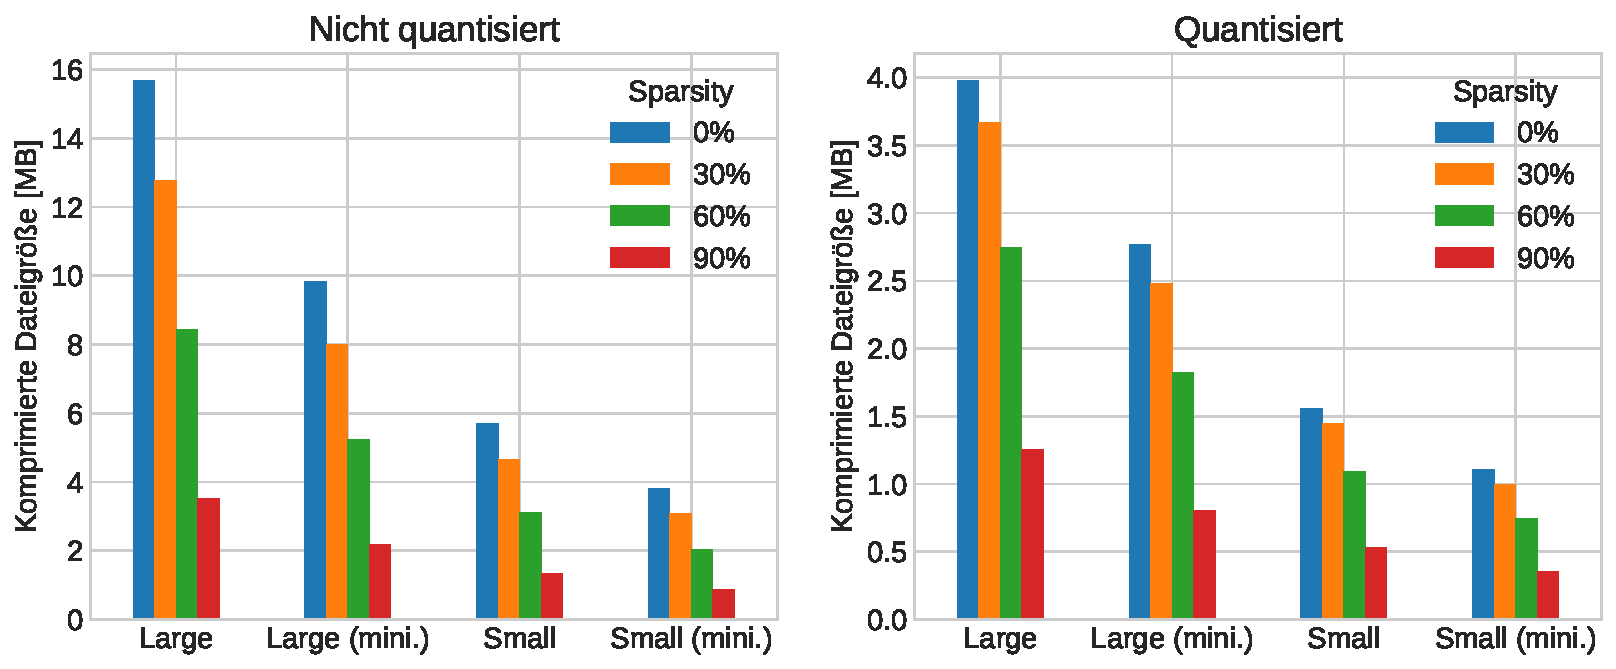
\includegraphics[width=\textwidth]{content/images/pruned_and_compressed_mnv3mini.pdf}}
\caption{Dateigröße für die MobileNetV3 Modelle mit $0\%$, $30\%$, $60\%$ und $90\%$ Sparsity nach Anwendung des gzip Kompressionsalgorithmus.}
\label{f4.11}
\end{figure}

Zusammengefasst haben die Verbesserungen der MobileNetV3 Architektur durch das Entfernen der Squeeze-And-Excitation Module, Austauschen der Hard-Swish Aktivierungsfunktion durch ReLU und die Reduzierung der Kernelgrößen in den Convolution-Schichten folgende Effekte ergeben:
\begin{itemize}
\item Das Entfernen der Squeeze-And-Excitation Module und das Ersetzen von $5 \times 5$ Convolutions durch $3 \times 3$ Convolutions hat die Anzahl an Parametern stark verringert und somit besitzen die Minimalistic-Varianten weniger Parameter und benötigen damit auch weniger Haupt- und Hintergrundspeicher.
\item Durch das Entfernen der Squeeze-And-Excitation Schichten, welche auf dem Rasp\-berry Pi 4 zu einer erhöhten Inferenzzeit geführt haben, konnte die Inferenzzeit auf dem Raspberry Pi 4 reduziert werden.
\item Möglicherweise hat das Austauschen der Hard-Swish Aktivierungsfunktion durch ReLU zu der verbesserten Genauigkeit beim Quantisieren der MobileNetV3 Minimalistic Architekturen im Gegensatz zu den normalen MobileNetV3 Architekturen geführt (siehe Abbildung \ref{f4.9}). Diese Vermutung ist damit begründet, da das Austauschen der Swish Aktivierungsfunktion durch ReLU6 bei den EfficientNet-lite Architekturen ebenfalls zu einer Verbesserung der Genauigkeit bei der Quantisierung geführt hat \cite{liu_higher_2020}.
\end{itemize}



\section{Diskussion}
In der bisherigen Arbeit wurden verschiedene Netzwerkarchitekturen auf dem CIFAR-10 Datensatz trainiert, ggf. mittels Pruning/Quantisierung optimiert und anschließend evaluiert. Bei der Diskussion der Ergebnisse der Evaluation hat sich herausgestellt, dass die einzelnen Architekturen teils sehr unterschiedlich auf die einzelnen Optimierungen reagieren. Den besten Trade-Off zwischen Genauigkeitsverlust und Kompression liefert in dieser Arbeit die MobileNet Architektur. Obwohl die MobileNet Architektur die älteste von den betrachteten Architekturen ist, hat sie, wie bereits in Abschnitt \ref{eval_quantisierung} gesehen, am stärksten von der Post-Training Quantisierung profitiert. Zusätzlich konnte die MobileNet Architektur beim Pruning und bei der Kombination aus Pruning und Quantisierung, mit zunehmender Sparsity, bessere Genauigkeiten erzielen als alle anderen betrachteten Architekturen. Durch die Kombination aus Pruning, Quantisierung und der Anwendung des gzip Kompressionsalgorithmus lässt sich der Speicherbedarf dieser Architektur auf 0.9MB verkleinern. Damit ist das MobileNet, bezogen auf den Hintergrundspeicherbedarf, nach der MobileNetV3 Small und MobileNetV2 Architektur, die drittkleinste Architektur. Wenn die Anwendung viel Wert auf eine hohe Genauigkeit legt und auf ein Pruning verzichtet werden kann, dann bieten sich statt der MobileNet Architektur die MobileNetV2 oder EfficientNet-B0 Architektur an. Die MobileNetV2 und EfficientNet-B0 Architektur haben im nicht-optimierten und quantisierten Zustand eine höhere Genauigkeit als die MobileNet Architektur. Jedoch sobald ein Pruning angewendet werden soll, geht der Genauigkeitsvorteil gegenüber der MobileNet Architektur verloren.
